
%%%%%%%%%%%%%%%%%%%%%%%%%%%%%%%%%%%%%%%%%%%%%%%%%%%%%%%%%%%%%%%%%%%%%%%%%%%%%%%%
%
% Analysis and Plotting
%
%%%%%%%%%%%%%%%%%%%%%%%%%%%%%%%%%%%%%%%%%%%%%%%%%%%%%%%%%%%%%%%%%%%%%%%%%%%%%%%%

\section{Analysis}
\label{sec:analysis}

%%%%%%%%%%%%%%%%%%%%%%%%%%%%%%%%%%%%%%%%%%%%%%%%%%%%%%%%%%%%%%%%%%%%%%%%%%%%%%%%


In this section, we discuss the details of the pipeline used for this work, including the analysis and plotting codes, databases, and automation scripts.  We also present an overview of the results obtained at each step.  A more in depth discussion of the observed trends and interpretations of results are presented in Sections~\ref{sec:2lpt--results} and \ref{sec:2lpt--discussion}.

As a high-level overview, we gather snapshots from previously run \lpt\ and \za\ simulations, find halos in each snapshot with \rockstar, match halos between simulations with \crossmatch, and compare the differences in various properties between corresponding \lpt\ and \za\ halos, primarily as functions of redshift and halo mass.  The specific codes developed for and used in our analysis are provided in the Appendices, and are referenced with the relevant discussions below.




%~~~~~~~~~~~~~~~~~~~~~~~~~~~~~~~~~~~~~~~~~~~~~~~~~~~~~~~~~~~~~~~~~~~~~~~~~~~~~~~
\subsection{Halo Properties with \rockstar}
\label{subsec:analysis--halo_properties}
%~~~~~~~~~~~~~~~~~~~~~~~~~~~~~~~~~~~~~~~~~~~~~~~~~~~~~~~~~~~~~~~~~~~~~~~~~~~~~~~


Halos are identified and measured with the \rockstar\ halo finder, which is discussed in detail in Section~\ref{sec:rockstar}.  Here, we discuss the setup necessary to run \rockstar, as well as its output files, post-processing steps, and particle list extraction.



%:::::::::::::::::::::::::::::::::::::::::::::::::::::::::::::::::::::::::::::::
\subsubsection{Simulation Snapshots and \rockstar\ Setup}
\label{subsubsec:analysis--halo_properties--output}
%:::::::::::::::::::::::::::::::::::::::::::::::::::::::::::::::::::::::::::::::


We run \rockstar\ on snapshots from each of our six simulation boxes.  Each box has 62 snapshots, with $512^{3}$ dark matter particles each.  Due to the large size of the snapshot data and the per-user disk space quota of the ACCRE cluster, only one box is able to be processed at a time.

For each snapshot, a \rockstar\ run directory is set up with a number of configuration files and scripts, including the \rockstar\ configuration file (Appendix~\ref{app:onenode}), PBS submission script (Appendix~\ref{app:run_rockstar}), a script to clean files from previous runs and begin a new run (Appendix~\ref{app:begin_run}), and a script for post-processing generated output files (Appendix~\ref{app:postprocess}).  A directory for particle data contains a link to the actual simulation snapshot and a file containing a list of snapshot files, which in this case contains one item.  A directory is also created for output halo data files.  We discuss automation of run directory setup and simultaneous launching of multiple \rockstar\ instances in Section~\ref{sec:automation}.

The parameter file controls various configuration options including simulation type, physical units, cosmological parameters, I/O options, halo definitions, and process setup.  \rockstar\ has native support for \gadget's snapshot format and can automatically import cosmological parameters and box size.  Length and mass scales must be input to convert from simulation units.  \rockstar\ uses periodic boundary conditions based on the number of analysis processes.  Periodic boundary conditions are assumed if using a multiple of eight analysis processes and are not assumed if using one analysis process.  For \rockstar\ to output BGC2 files (discusses below in Section~\ref{subsubsec:analysis--halo_properties--output}), the path of a file containing a list of snapshot filenames must be set as the BGC2 snapnames option.  Halo virial radius and mass definitions may be set to either virial or a multiple of either the critical or background density.  We select halos to be defined by the virial radius and mass.  We are interested in defining halos as spherical overdensity halos rather than friends-of-friends halos, so we also choose to define halo properties based on all particles within the virial radius, whether or not they are energetically bound to the halo.

\rockstar\ is run as a server-client setup.  This is designed so that one processor acts as a director and output manager, one or more processors read in the input snapshots, and the remaining processors or compute nodes do the actual processing on different segments of the simulation box.  \rockstar\ uses sockets for communication between the server process and the worker processes if running on multiple nodes.  However, we were unable to configure \rockstar\ in a way that it would run across multiple compute nodes, so we run each instance of \rockstar\ on one node, with ten processor cores for the necessary functions.  One processor acts as the server, one as the snapshot reader, and the remaining eight as halo finders.



%:::::::::::::::::::::::::::::::::::::::::::::::::::::::::::::::::::::::::::::::
\subsubsection{\rockstar\ Output and Post-processing}
\label{subsubsec:analysis--halo_properties--output}
%:::::::::::::::::::::::::::::::::::::::::::::::::::::::::::::::::::::::::::::::


\rockstar\ outputs halo information in ASCII plaintext, binary, and BGC2 binary formats.  As mentioned above, we run \rockstar\ with eight worker processes per snapshot.  Each worker process outputs it's own set of data files, with each file covering a separate octant of the simulation box plus a small overlap region.  Halos with particles in the overlap region are saved based on the location of their centers.  In addition to the per-processor output, a composite list of halos (and only halos) from all worker processors are created.

Through its various output files, \rockstar\ provides a large number of measured halo properties.  Whether or not full friends-of-friends particle lists are saved is controlled via the configuration file.  Spherical overdensity particle lists are saved when utilizing BGC2 output.  Particle data include particle ID, position, and velocity.  Particle mass is not included as our simulations have uniform particle mass.  Halo information consists of a large number of parameters, including halo ID, number of constituent particles, masses to various radii, position, velocity, angular momentum, spin, virial radius, scale radius, shape parameters, energy parameters, position and velocity offsets between the center of mass and the peak density, and parent halo ID.

As previously mentioned, we want halos defined based on spherical overdensity particle lists.  These are only available from \rockstar's BGC2 binary output format, with all other available particle lists consisting of friends-of-friends particles.  The BGC2 files consist of a 1024 byte header, halo data of 72 bytes per halo, and particle data with 32 bytes per particle.  The header consists of an unsigned 8-byte integer, 16 8-byte signed integers, 19 8-byte double-precision floating point numbers, and extra padding out to 1024 bytes.  The halo data consists of 2 8-byte signed integers, 2 8-byte unsigned integers, and 10 4-byte floating point numbers per halo.  The particle data consists of 1 8-byte signed integer and 6 4-byte floating point numbers per particle.  There is a 4-byte offset before the header, and 8-byte offsets between the header and halo data and between the halo data and particle data.  The reader is referred to the bgc2.h header of the \rockstar\ source code for further information on the contents of each structure.  Our python code for reading in BGC2 files is presented in Appendix~\ref{app:bgc2}.  C code for reading in BGC2 files is bundled with the \rockstar\ source code.

After \rockstar\ is run, some post-processing of the output is needed.  By default, \rockstar\ does not provide information on membership information for substructure.  Two scripts---one for the composite halo list and one for the BGC2 files---are provided with \rockstar\ to cycle back through the halo lists and find the "parents," or the halo in which a given subhalo is contained.  A script is also provided to convert halo information in the BGC2 files to ASCII plaintext.  Our script for running these post-processing steps is presented in Appendix~\ref{app:postprocess}.




%~~~~~~~~~~~~~~~~~~~~~~~~~~~~~~~~~~~~~~~~~~~~~~~~~~~~~~~~~~~~~~~~~~~~~~~~~~~~~~~
\subsection{Density Profile Fitting}
\label{subsec:analysis--profile_fitting}
%~~~~~~~~~~~~~~~~~~~~~~~~~~~~~~~~~~~~~~~~~~~~~~~~~~~~~~~~~~~~~~~~~~~~~~~~~~~~~~~


While \rockstar's output includes measurements for halo virial and scale radii, and thus concentration, we independently fit NFW density profiles to halos and measure concentration as a verification of \rockstar's fitting.  The full density profile python code is presented in Appendix~\ref{app:density_profile}.  This section is included for completeness only, as we find that only a small fraction of halos are well fit by our method, and we instead rely on concentration measurements directly from \rockstar\ for subsequent analysis.



%:::::::::::::::::::::::::::::::::::::::::::::::::::::::::::::::::::::::::::::::
\subsubsection{Density Profiles}
\label{subsubsec:analysis--profile_fitting--density_profiles}
%:::::::::::::::::::::::::::::::::::::::::::::::::::::::::::::::::::::::::::::::


For each halo, a list of constituent spherical overdensity particles is obtained from the post-processed BGC2 catalog from \rockstar's output.  For our purposes here, the relevant parameters are particle mass and position.  We also use the values for each halo's center position and virial radius as found by \rockstar.

Density profiles are then constructed by binning the particle positions in logarithmic radial bins from the resolution limit of the simulation to the halo virial radius and multiplying by particle mass.  Before being passed to the fitting routine, density profiles are normalized to unity for both virial radius and maximum density. 



%:::::::::::::::::::::::::::::::::::::::::::::::::::::::::::::::::::::::::::::::
\subsubsection{Fitting}
\label{subsubsec:analysis--profile_fitting--fitting}
%:::::::::::::::::::::::::::::::::::::::::::::::::::::::::::::::::::::::::::::::


Halos are fit using the CurveFit routine from the SciPy Optimize library.  It uses the Levenberg-Marquardt algorithm \citep{1963SIAM...11...431} for non-linear least squares fitting.

CurveFit is called by providing a model function, independent variable, measured dependent variable, and optionally weights for the dependent variable and initial guesses for fit coefficients.  Here, our fit function is the NFW dark matter density profile (see Equation~\ref{eq:nfw_profile}).  The free parameters to be fit are the scale radius $R_{s}$ and the characteristic density $\rho_{0}$.

As the least squares algorithm is sensitive to local minima, care must be taken in choosing initial guesses for the fit coefficients.  Additionally, large dynamic range in the fit parameters tended to produce poor results.  We explored a number of solutions to improve solution stability, including fitting in logarithmic space and randomizing the initial guesses and picking the best solution.  We found the best results were achieved by normalizing the data to unity for both radius and density, and choosing initial guesses within an order of magnitude for a typical halo, namely, normalized $R_{s} = 0.1$ and normalized $\rho_{0} = 1.0$.

Some halos with irregular profiles presented the problem of the fitting algorithm choosing an unphysical scale radius larger than the virial radius of the halo.  In order to heavily penalize this option from being chosen by the fitting algorithm, the dependent variable returned by the model function must differ from the input measured dependent variable as much as possible.  However, we discovered that the transition must also be smooth, as a disjointed jump such as, say, returning a very large number for every value if $R_{s} > R_{\mathrm{vir}}$ would cause the algorithm to fail.  We achieve this smooth transition penalty by adding the term $(R_{s} - 1) e^{r}$ to the density returned by the model function if the fitting algorithm tries to guess a value of $R_{s}$ larger than $R_{\mathrm{vir}}$.  However, while this did force halos to have definable concentrations, these halos often ended up with best fit scale radii equal to or just slightly less than the virial radii.

As we fit halos over a large range in redshift, we found low particle count halos to have noisy density profiles that were inherently more difficult to properly fit.  Throughout our analysis, we use a lower bound of 100 particles to define a halo.  At high redshift, even the largest halos are just beginning to cross this threshold.  With such few particles spread across the number of bins necessary to properly define a density profile, we are left with only a handful of particles per bin.  In Figure~\ref{fig:fitting--density_profiles}, we compare one of the largest halos at $z = 14$ with one of the largest halos at the end of the simulation at $z = 6$.

\begin{figure}[t]
	\centering
	\begin{subfigure}{}
		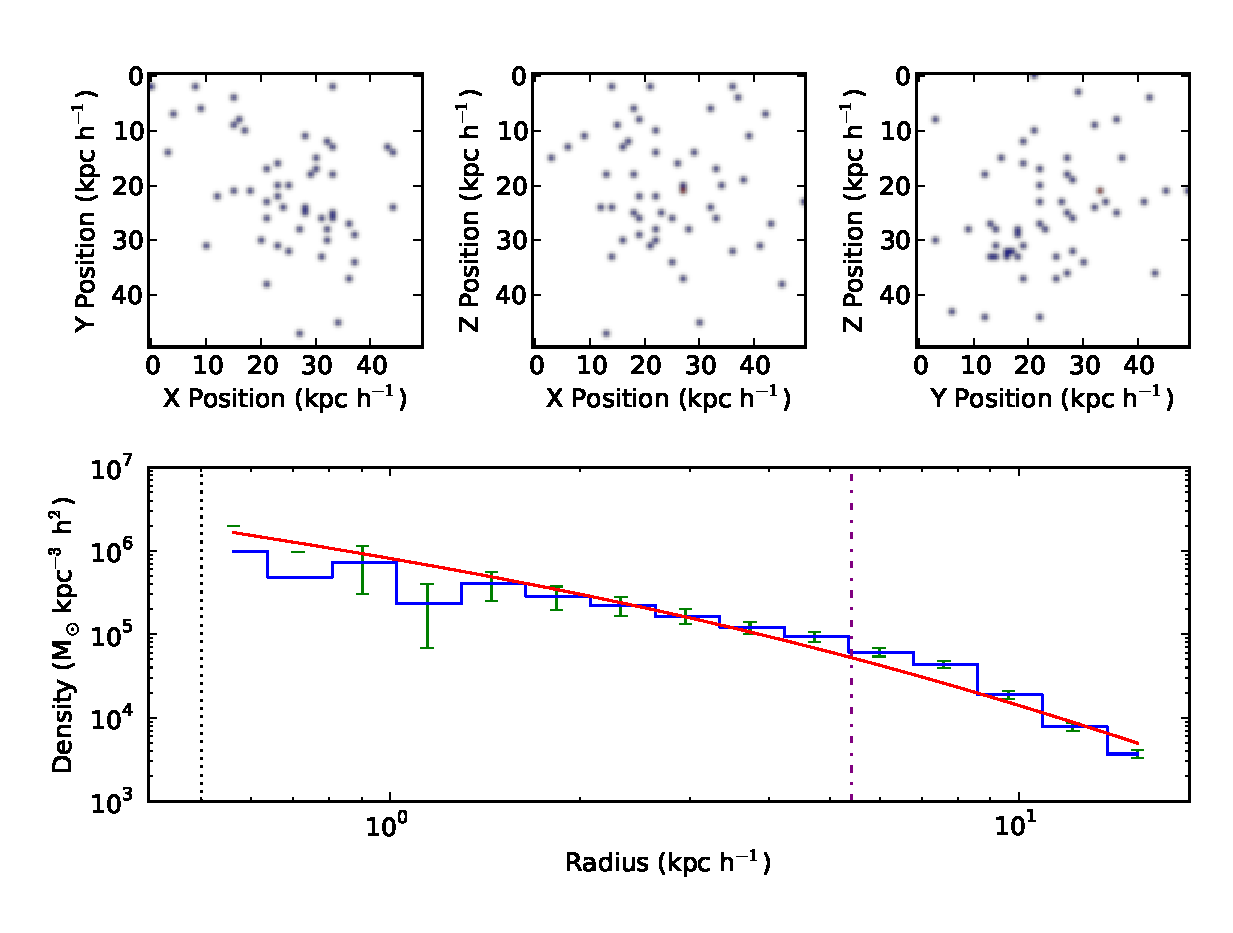
\includegraphics[width=0.75\linewidth]{analysis/2lpt_040_density_profile_0.eps}
	\end{subfigure}
	\\
	\begin{subfigure}{}
		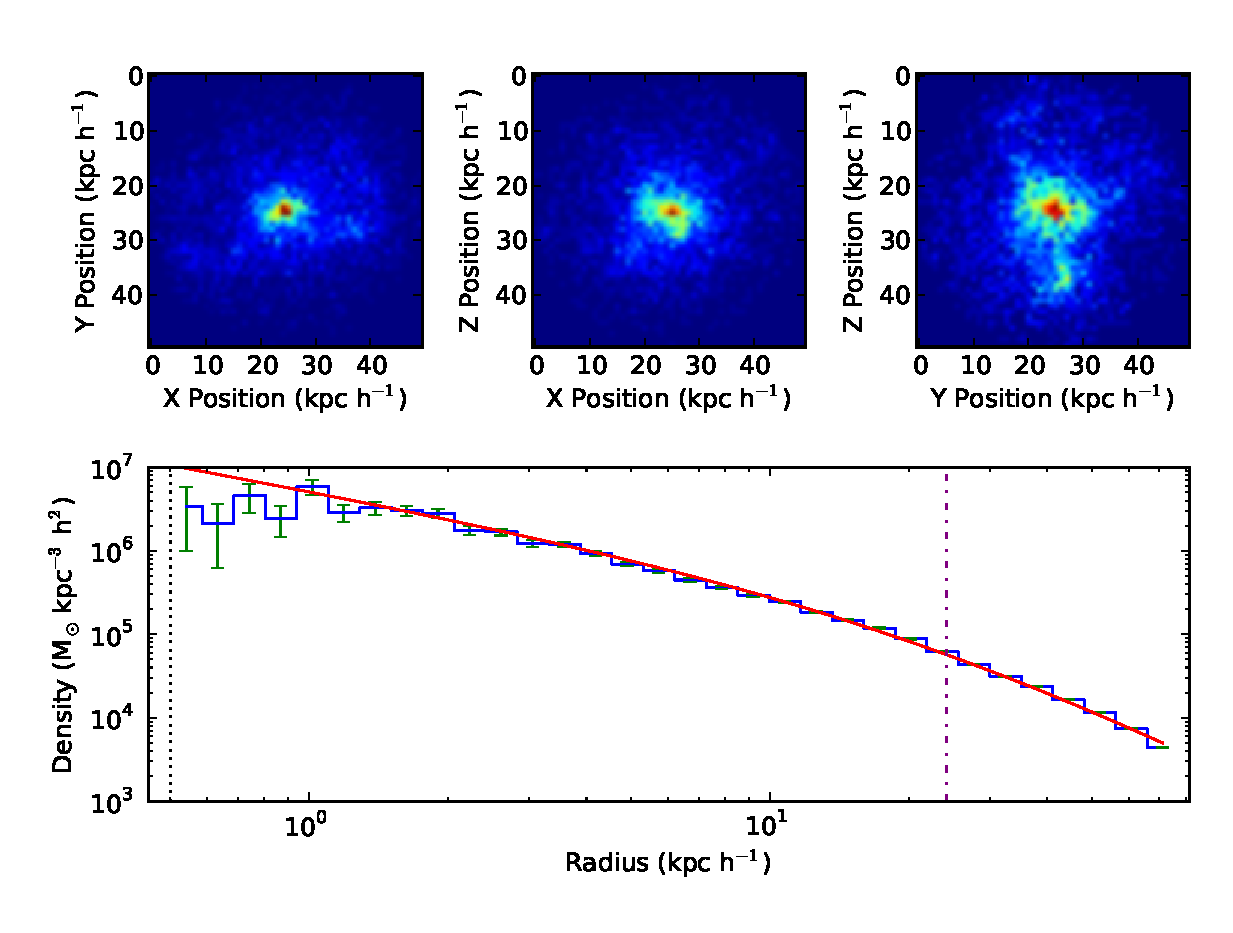
\includegraphics[width=0.75\linewidth]{analysis/2lpt_061_density_profile_0.eps}
	\end{subfigure}
	\caption[Density profiles for two large halos at $z = 14$ and $z = 6$.]{\footnotesize Density profiles for two large halos at $z = 14$ and $z = 6$.  Both halos are from the Box 1 \lpt\ simulation, and are the largest halos at their respective redshifts.  \mrk{(Get rid of density projections.)}}
	\label{fig:fitting--density_profiles}
\end{figure}



%:::::::::::::::::::::::::::::::::::::::::::::::::::::::::::::::::::::::::::::::
\subsubsection{Characterization of Uncertainty}
\label{subsubsec:analysis--profile_fitting--uncertainty}
%:::::::::::::::::::::::::::::::::::::::::::::::::::::::::::::::::::::::::::::::


An initial motivation for finding our own concentration parameters independent from \rockstar\ is that \rockstar\ does not provide information about the quality of its density profile fits.  We assign Poisson errors to the density in each bin such that $\sigma_{\rho} = \rho \sqrt{N} / N$, where $\rho$ is the density and $N$ is the number of particles in each bin.  These uncertainties are then provided as weights to the CurveFit routine.  Upon finding a best fit, the routine provides the fit parameters and an estimation of the uncertainty in those parameters via a covariance matrix, which we use to uncertainty in the concentration.  Additionally, we find the $\chi^{2}$ for the overall fit, which we use as an indicator of whether to accept or reject the fit for a given halo.



%:::::::::::::::::::::::::::::::::::::::::::::::::::::::::::::::::::::::::::::::
\subsubsection{Mass Profiles}
\label{subsubsec:analysis--profile_fitting--mass_profiles}
%:::::::::::::::::::::::::::::::::::::::::::::::::::::::::::::::::::::::::::::::


Text goes here.  Mass profiles tested to avoid binning issues and the stats stuff Manodeep learned at the conference.  Bad fitting results, so abandoned.  Figure~\ref{fig:mass_profile}.

\begin{figure}[t]
	\centering
	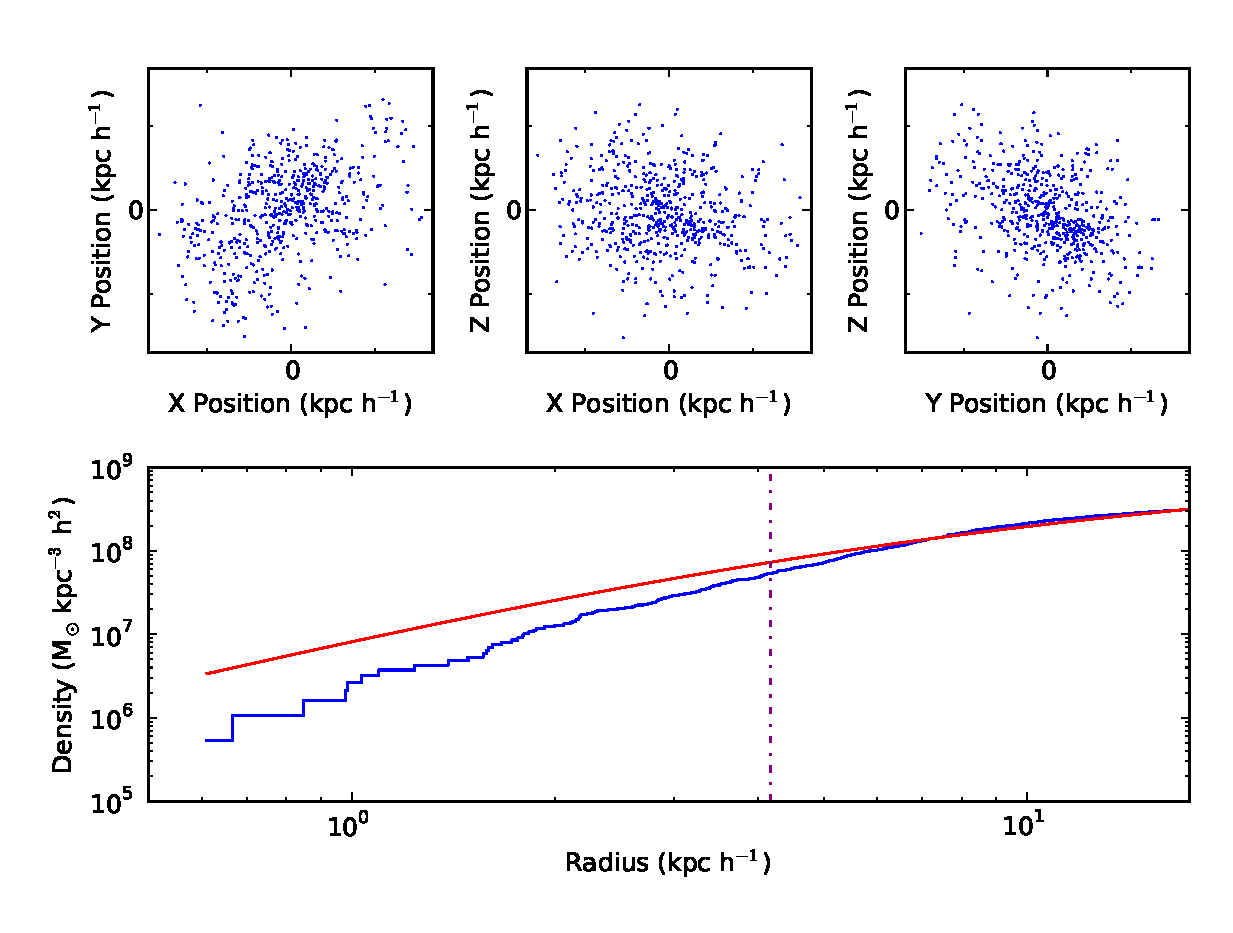
\includegraphics[width=\linewidth]{analysis/2lpt_061_mass_profile_0.eps}
	\caption[Mass profiles a large halo at $z = 6$.]{\footnotesize Mass profiles for a large halo at $z = 6$.  \mrk{(Get rid of density projections.)}}
	\label{fig:mass_profile}
\end{figure}



%:::::::::::::::::::::::::::::::::::::::::::::::::::::::::::::::::::::::::::::::
\subsubsection{Concentration Comparison to \rockstar}
\label{subsubsec:analysis--profile_fitting--rockstar_comparison}
%:::::::::::::::::::::::::::::::::::::::::::::::::::::::::::::::::::::::::::::::


Overall, we do not find good agreement with \rockstar.  Using a script (see Appendix~\ref{app:concentration_comparison}) to compare the concentrations derived from our fits with those from \rockstar.  At $z = 6$, we find that only 26\% of halos fit by our method have concentrations within 20\% of concentrations as measured by \rockstar.  We have slightly more agreement with high mass halos, with 37\% agreement if we only consider the most massive 10\% of halos.  Additionally, we do not find good fits for every halo.  If the distribution of particles would produce too few bins or the fitting routine exceeded a maximum number of iterations to find a stable solution, the halo is not fit.  We also exclude halos with fits returned with very large $\chi^{2}$ values.  Because of the discrepancies in our results and the fact that we do not find acceptable fits for every halo, we use the more complete \rockstar\ data for the final concentration measurements used in the remainder of our analysis.




%~~~~~~~~~~~~~~~~~~~~~~~~~~~~~~~~~~~~~~~~~~~~~~~~~~~~~~~~~~~~~~~~~~~~~~~~~~~~~~~
\subsection{Cross-matched Halo Catalog}
\label{subsec:analysis--catalog}
%~~~~~~~~~~~~~~~~~~~~~~~~~~~~~~~~~~~~~~~~~~~~~~~~~~~~~~~~~~~~~~~~~~~~~~~~~~~~~~~


With halo catalogs generated by \rockstar\ for both \lpt\ and \za\ simulations, we need to be able to directly compare corresponding halos from the two suites of simulations.  We match halos between simulations based on constituent particles with the \crossmatch\ code modified to import \rockstar's BGC2 binary output files.  Properties of the matched halos are then compiled into one large database per box for further filtering and analysis.



%:::::::::::::::::::::::::::::::::::::::::::::::::::::::::::::::::::::::::::::::
\subsubsection{Cross-matching}
\label{subsubsec:analysis--catalog--crossmatching}
%:::::::::::::::::::::::::::::::::::::::::::::::::::::::::::::::::::::::::::::::


Our simulations are initialized with identical particle ID schemes, and we are thus able to uniquely identify and track matching particles between simulations and match halos based on the largest number of shared particles.  As the full implementation of the \crossmatch\ code is previously discussed in Section~\ref{sec:crossmatch}, we only briefly summarize its place in our analysis pipeline here.  The script in Appendix~\ref{app:crossmatch_setup} sets up the directory structure for the \crossmatch\ analysis and copies the \crossmatch\ parameter files (Appendices~\ref{app:crossmatch_2lpt_config} and \ref{app:crossmatch_za_config}) to the appropriate run directories.  \crossmatch\ is then run for each snapshot via the submission script in Appendix~\ref{app:run_crossmatch}, which is run for each simulation box.

Once caveat of the \crossmatch\ code is that matches are not necessarily unique.  For each halo in the first simulation, only one best match halo will be selected from the second simulation.  However, there may be other halos from the first simulation that also have the same halo from the second simulation selected as a best match.  To counter this, we run \crossmatch\ in both directions---once matching \za\ halos to \lpt\ halos and once matching \lpt\ halos to \za\ halos---and choose best match halos as those that are matched in both directions.  This assures a unique one-to-one matching between \lpt\ and \za\ halos.  The code and submission script that select the best matches from the \lpt-first and \za-first cross-matched halo lists are presented in Appendix~\ref{app:best_match}.



%:::::::::::::::::::::::::::::::::::::::::::::::::::::::::::::::::::::::::::::::
\subsubsection{Database Aggregation and Filtering}
\label{subsubsec:analysis--catalog--aggregation}
%:::::::::::::::::::::::::::::::::::::::::::::::::::::::::::::::::::::::::::::::


We now have raw halo data we need for further study, but are also left with a large number of disparate files that contain this information.  For every snapshot, we have cross-simulation halo matching information from \crossmatch\ and the best match selection script, independent density profile and concentration measurement information from the density profile program, and original halo properties and host halo membership information from \rockstar\ spread across plaintext and BGC2 binary files for each processor on which \rockstar\ was run, all for three simulation boxes each for both \lpt\ and \za.

We combine the information from all of these file into one centralized database per snapshot with the database generation program and submission script in Appendix~\ref{app:database_generation}.  The program reads in all of the source data files, finds companion halos from the output of \crossmatch, and outputs all available data for each halo pair aggregated together.  The program is run for each of our 62 snapshots per simulation box, giving 186 total database files.

With the first version of our database generation code, total runtime became a significant factor.  The halo matching code was initially implemented in a naive double loop search through all the data files to find collect halo pair properties.  Pure python loop structures are exceedingly slow for larger data sets, and an initial estimate gave a runtime on the order of weeks or months.  This was unacceptable, as there are many snapshots, and the aggregation may need to be performed multiple times if any of the previous steps in the analysis pipeline were to be modified.  The code was therefore rewritten to take full advantage of the vectorization of the NumPy library, achieving a massive speedup to a runtime of order a few seconds.

In order to retain a centralized database of all available information for matched halos, we do not filter out halos at this step.  Subsequent analysis, however, does remove halo pairs from consideration in certain circumstances.  For early analysis involving our independent density profile fitting, we remove halos based on evidence of a poor fit, including halos that have measured concentrations greater than 100 or less than 1, $\rho_{0}$ less than zero, or $\chi^{2}$ greater than 10.  For all analysis, we remove halos with fewer than 100 particles and halos that exist as substructure in a larger host halo.




%~~~~~~~~~~~~~~~~~~~~~~~~~~~~~~~~~~~~~~~~~~~~~~~~~~~~~~~~~~~~~~~~~~~~~~~~~~~~~~~
\subsection{Halo Comparison}
\label{subsec:analysis--halo_comparison}
%~~~~~~~~~~~~~~~~~~~~~~~~~~~~~~~~~~~~~~~~~~~~~~~~~~~~~~~~~~~~~~~~~~~~~~~~~~~~~~~


With a catalog of DM halos cross-matched between \lpt\ and \za\ simulations, we are able to directly compare properties on a halo-by-halo basis.  At this stage, we are mostly concerned with a qualitative comparison between individual halos in order to judge the overall success of halo matching and the broad differences in halo evolution arising from differences in simulation initialization.



%:::::::::::::::::::::::::::::::::::::::::::::::::::::::::::::::::::::::::::::::
\subsubsection{Match Verification}
\label{subsubsec:analysis--halo_comparison--match_verification}
%:::::::::::::::::::::::::::::::::::::::::::::::::::::::::::::::::::::::::::::::


In order to compare halo evolution between \lpt\ and \za\ simulations, we first need to ensure that the halos being compared do actually represent the same halo in each simulation.  The \crossmatch\ code as well as its implementation in our analysis pipeline are discussed above, so here we instead focus on the plots used as a visual sanity check on the resulting matches.  The python code used to generate these plots is listed in Appendix~\ref{app:particle_comparison}.

As we wish to compare halos that may have followed different evolutionary paths in their respective \lpt\ or \za\ simulations, we are unable to do a hard cut on a single parameter such as mass, radius, position or particle distribution.  However, large variances in any of these properties can hint at a problem in the matching algorithm.  We therefore perform a quick visual check on a number of halo pairs by plotting their relative positions, radii, and constituent particle distributions in order to verify that the \crossmatch\ code performed as expected.

An example of this comparison is shown in Figure~\ref{fig:match_verification}, where we plot two large matching halos at $z = 6$.  Particles belonging to the halos are plotted as points, with \lpt\ halo particles in blue and \za\ halo particles in red.  The virial radii of the two halos are represented by the black circles.  The virial radii and particle distributions are very similar, and there is only a small offset in position.  We consider this a successful match.

\begin{figure}[t]
	\centering
	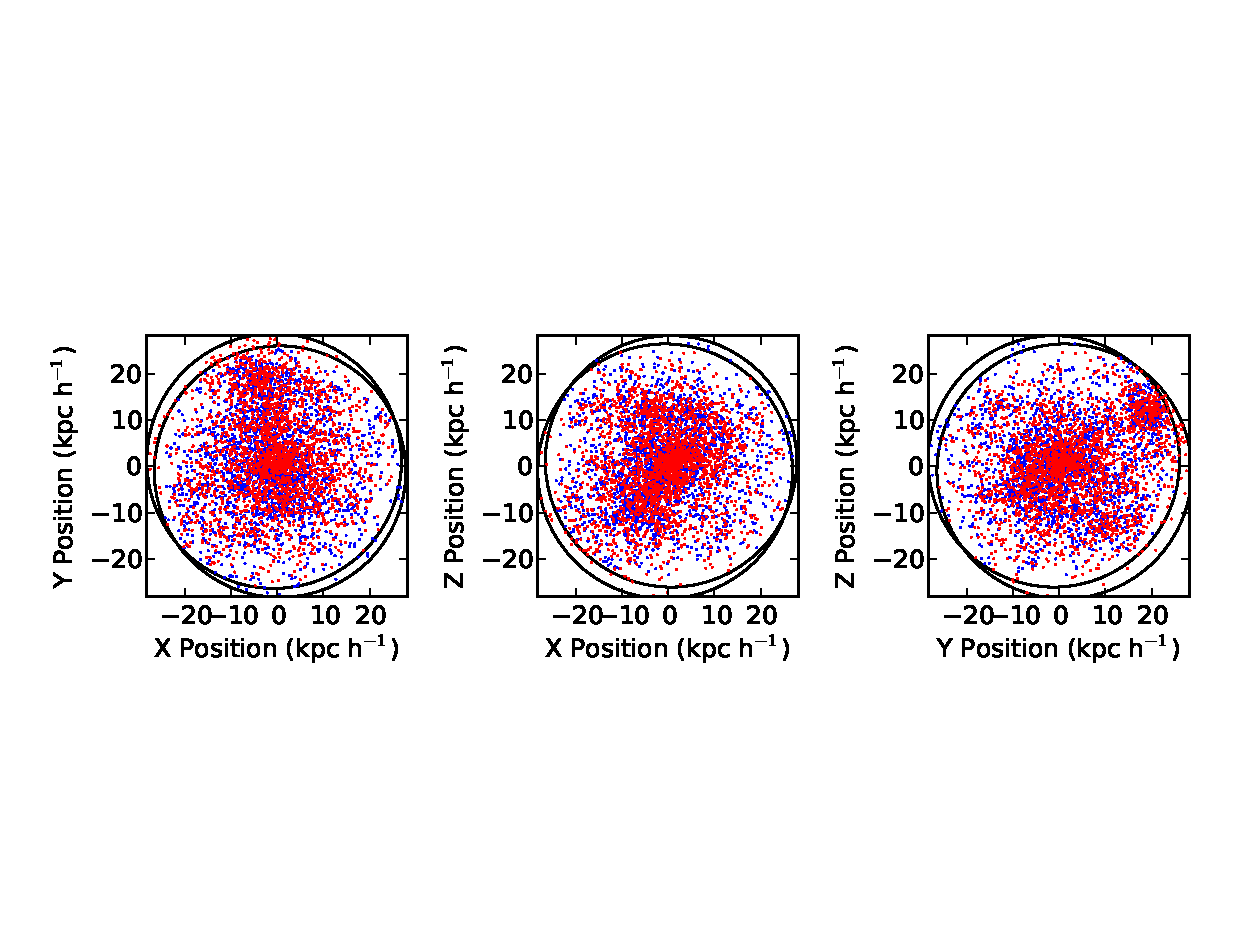
\includegraphics[width=\linewidth]{analysis/match_particles.eps}
	\caption[Example of halo particle matching at $z = 6$.]{\footnotesize Example of halo particle matching at $z = 6$.  Blue dots are \lpt\ halo particles, and red dots are \za\ halo particles.  Black circles are the virial radii of the halos.  Good matches are achieved for halos, with only slight drift between simulations.}
	\label{fig:match_verification}
\end{figure}



%:::::::::::::::::::::::::::::::::::::::::::::::::::::::::::::::::::::::::::::::
\subsubsection{Morphology}
\label{subsubsec:analysis--halo_comparison--morphology}
%:::::::::::::::::::::::::::::::::::::::::::::::::::::::::::::::::::::::::::::::


The morphology of a dark matter halo can provide insight into its structural evolution and merger history.  Features such as tidal features, irregular shapes, and offset nuclei hint at recent merger activity, while more symmetrical distributions suggest a quieter recent history.  We compare DM particle distributions of matched halos by observing the projected density map along three axis vectors.  The python code for plotting these, as well as the density profiles discussed below, is listed in Appendix~\ref{app:density_comparison}.

By comparing the projected density morphologies of companion \lpt\ and \za\ halos, we get a qualitative impression of the differences in their current evolutionary state.  We found the inner nuclear region to often display the most discernible difference in structure between the two halos.  For halo pairs where this difference is most apparent, such as one halo having a single central core with the other halo having two distinct density peaks, we believe the most likely cause to be an offset in merger epochs between the two simulations.  In this case, the snapshot from one simulation would catch the merger in progress, with multiple unsettled density peaks still visible, while the other simulation snapshot would catch the halo after it has settled into a more virialized state.

As an example of this, we plot comparisons of two $z = 6$ halo pairs in Figures~\ref{fig:density_comparison_000} and~\ref{fig:density_comparison_070}.  The top two rows of panels of each show XY, XZ, and YZ projections of the dark matter density for the \lpt\ and \za\ halo on the first and second row, respectively.  The density map is shown with a logarithmic color scale, and equal density contours are marked with white curves.  Figure~\ref{fig:density_comparison_000} shows a pair of large halos that display similar central structure.  These halos are unlikely to have largely differed in their evolution shortly prior to the snapshot.  Figure~\ref{fig:density_comparison_070}, however, shows a halo pair with differing nuclear structure.  The \za\ halo displays two distinct central density peaks, while the \lpt\ halo shows only a single more relaxed core.

\begin{figure}[t]
	\centering
	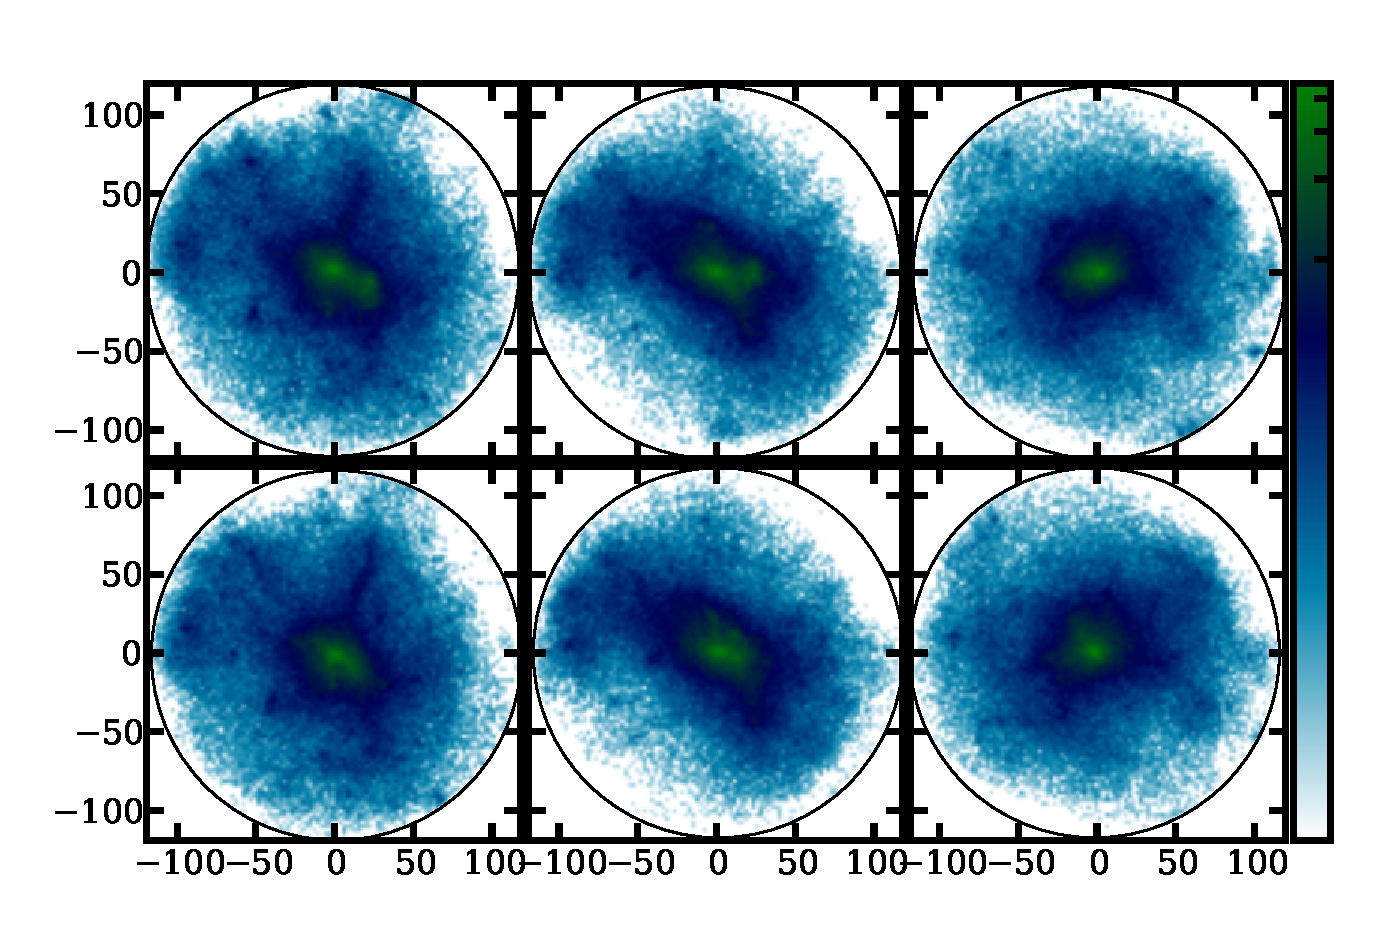
\includegraphics[width=0.75\linewidth]{analysis/halo-pair_000_snap061.eps}
	\caption[Comparison of two large well-fit companion halos $z = 6$.]{\footnotesize Two large matched halos at $z = 6$ with similar nuclear structure.  \emph{Top two rows:}  Projected density maps, with XY, XZ, and YZ views of the central nuclear region of the halos.  Density is represented by a logarithmic color scale, and equal density contours are plotted as white curves.  The first and second rows depict the \lpt\ and \za\ halo, respectively.  \emph{Bottom two rows:}  Radially-binned halo density profiles fit with the NFW density profile model.  The blue stepped profiles are the binned data, red curves are the fit NFW models, black dashed lines are the resolution limit of the simulation, and purple dot-dash lines are the measured scale radius.}
	\label{fig:density_comparison_000}
\end{figure}

\begin{figure}[t]
	\centering
	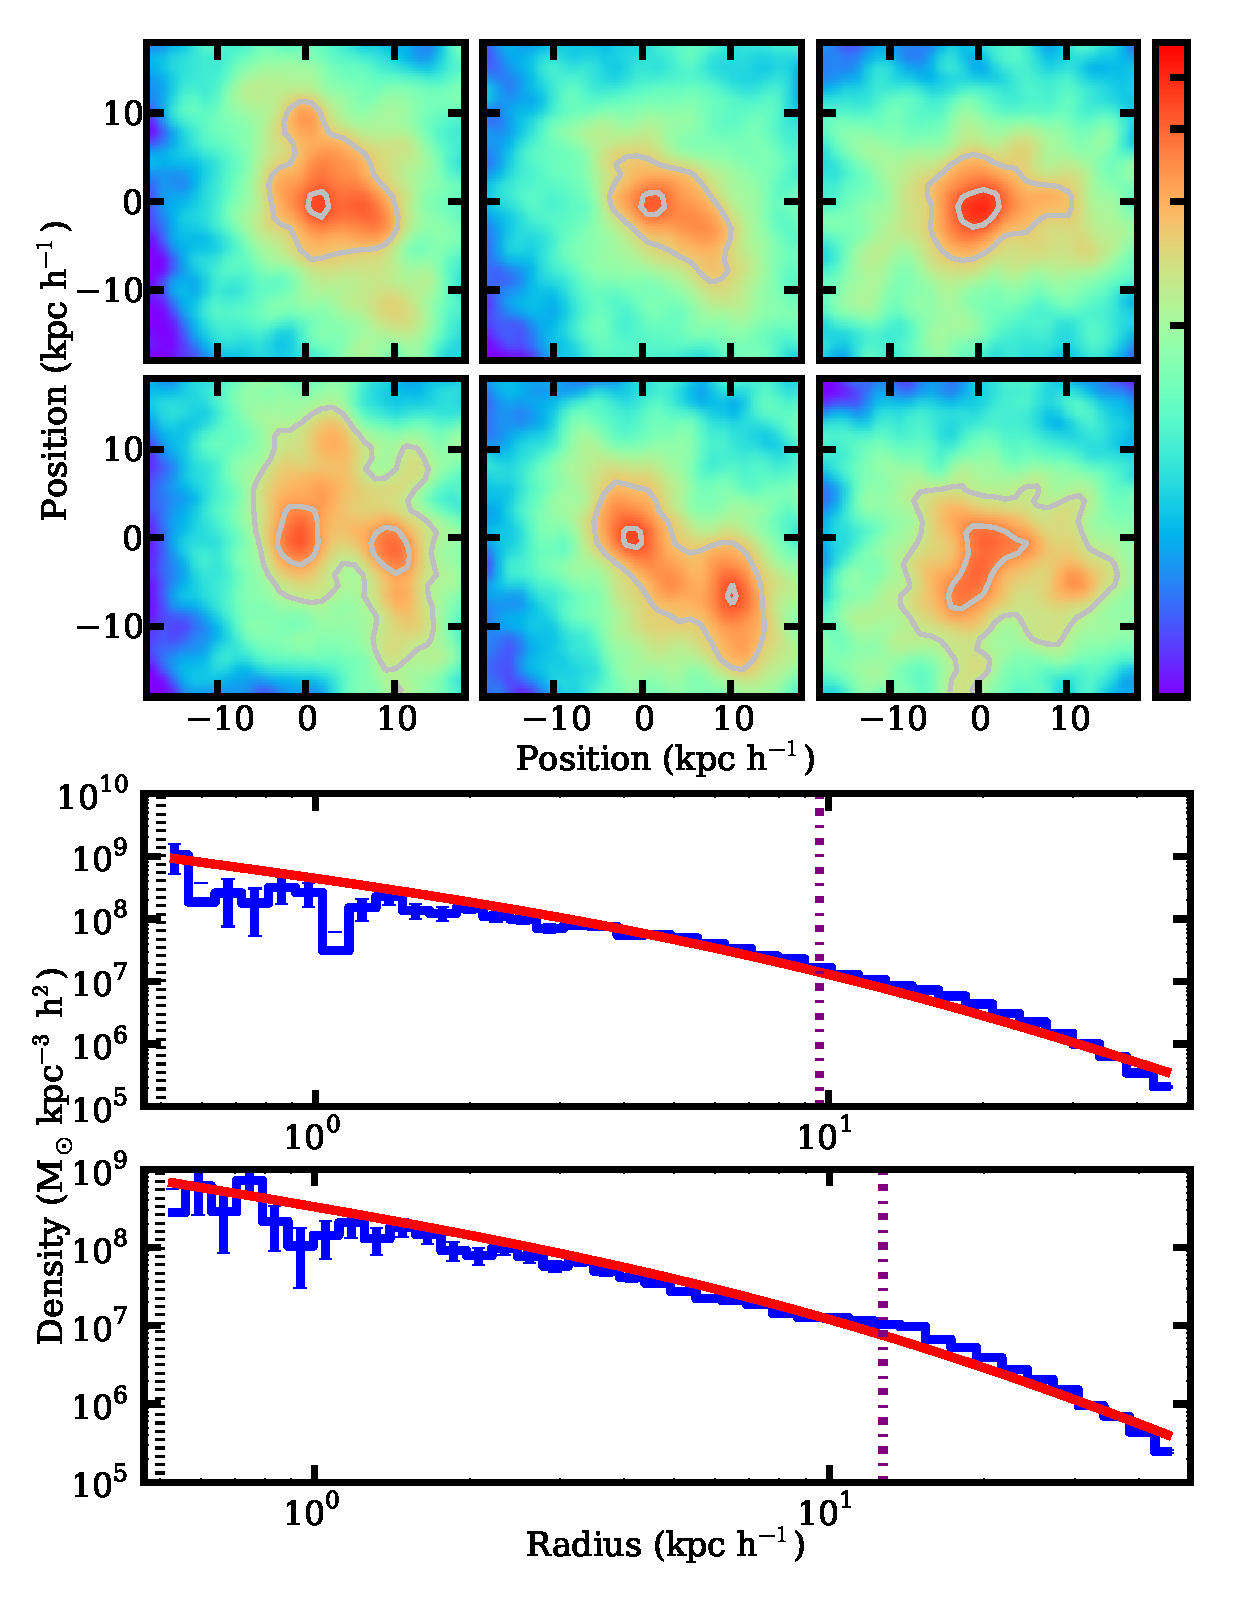
\includegraphics[width=0.75\linewidth]{analysis/halo-pair_070_snap061.eps}
	\caption[Comparison of two large companion halos $z = 6$ with differing nuclear structure.]{\footnotesize Like Figure~\ref{fig:density_comparison_000}, but for two large matched halos at $z = 6$ with differing nuclear structure.}
	\label{fig:density_comparison_070}
\end{figure}



%:::::::::::::::::::::::::::::::::::::::::::::::::::::::::::::::::::::::::::::::
\subsubsection{Density Profiles}
\label{subsubsec:analysis--halo_comparison--density_profiles}
%:::::::::::::::::::::::::::::::::::::::::::::::::::::::::::::::::::::::::::::::


The code listed in Appendix~\ref{app:density_comparison}, which produces the density projections discussed above, also plots comparisons of the halos' density profiles.  We have addressed the creation of density profiles in Section~\ref{subsec:analysis--profile_fitting}, and here the same method is used for each profile.  In this case, we with to directly compare the profiles of the companion \lpt\ and \za\ halos, so they are plotted together, alongside the 2-D density projections discussed in the previous section.

We again consider the halo pairs compared in Figures~\ref{fig:density_comparison_000} and~\ref{density_compairson_070}, where the bottom two panels of each display the density profiles of the \lpt\ and \za\ halos, respectively.  Halo particles are binned in logarithmically-spaced radial bins from the virial radius inward to the simulation resolution limit.  The profiles are fit with the NFW profile model with free parameters for scale radius and characteristic density.  The resulting fit is overplotted as red curves, and the scale radius is marked with the vertical purple dot-dash lines.

The halos in Figure~\ref{fig:density_comparison_000} display very similar central morphology and are both well-fit by the NFW profile.  The more relaxed and spherically symmetrical halos such as these tend to be easier to fit well than more irregular halos.  The measured scale radii for these halos are also very similar, and combined with the similar virial radii, produce similar concentration values.  The halos in Figure~\ref{fig:density_comparison_070} display a more differing structure.  While the \lpt\ halo is relatively symmetrical, allowing it to be relatively well-fit by the NFW model, the \za\ halo has two distinct central density peaks, causing the NFW fit to be a bit less accurate.  Here, there is a marked difference in the resulting scale radii, with the \lpt\ halo displaying a larger concentration than its \za\ companion.




%~~~~~~~~~~~~~~~~~~~~~~~~~~~~~~~~~~~~~~~~~~~~~~~~~~~~~~~~~~~~~~~~~~~~~~~~~~~~~~~
\subsection{Difference Distributions}
\label{subsec:analysis--difference_histograms}
%~~~~~~~~~~~~~~~~~~~~~~~~~~~~~~~~~~~~~~~~~~~~~~~~~~~~~~~~~~~~~~~~~~~~~~~~~~~~~~~


We now turn our focus to the ensemble halo population as a whole.  Comparing individual companion halos can realistically only give a qualitative picture of differences arising between \lpt\ and \za\ simulations, as the large number of halos necessitates consideration of only a small percentage of the sample.  We therefore need a consistent way of measuring the behavior of the entire population.  In this section, we discuss how we measure these differences in halo populations using the codes listed in Appendix~\ref{app:diff_hist}.  In particular, the analysis code itself is listed in Appendix~\ref{app:hist}, the script to run the analysis on the combined halo population from all three simulation boxes is listed in Appendix~\ref{app:run_diff_hist}, the script to run the analysis on the simulation boxes independently is listed in Appendix~\ref{app:run_diff_hist_individual_boxes}, and the script to collect the resulting statistics from all the individual snapshots into one database is listed in Appendix~\ref{app:collect_stats}.



%:::::::::::::::::::::::::::::::::::::::::::::::::::::::::::::::::::::::::::::::
\subsubsection{Histograms}
\label{subsubsec:analysis--difference_histograms--binning}
%:::::::::::::::::::::::::::::::::::::::::::::::::::::::::::::::::::::::::::::::


We wish to explore differences in a number of halo properties, so we construct a generic distribution so that any measured halo quantity $q$ can be considered.  The distribution should  highlight the differences between \lpt\ and \za\ halo populations while remaining unbiased to the choice of simulation initialization.  This leaves us with a distribution of the differences between \lpt\ and \za\ quantities, normalized by the average of the two:
\begin{equation} \label{eq:delta_q}
	\Delta q = \frac{q_{\lpt} - q_{\za}}{q_{\mathrm{avg}}},
\end{equation}
where $q_{\mathrm{avg}} = \frac{1}{2} (q_{\lpt} + q_{\za})$.  Defined in this way, difference distributions of, e.g.,  virial mass $\Delta \Mvir$, concentration $\Delta c$, or the offset distance between the central density peak and the center of mass $\Delta \Xoff$ can all be considered on equal footing.  We create distribution histograms of $\Delta q$ for various halo quantities both for the combined halo catalog from the stacked simulation boxes and for the individual simulation boxes separately.


%:::::::::::::::::::::::::::::::::::::::::::::::::::::::::::::::::::::::::::::::
\subsubsection{Fitting}
\label{subsubsec:analysis--difference_histograms--fitting}
%:::::::::::::::::::::::::::::::::::::::::::::::::::::::::::::::::::::::::::::::


In order to extract a number of statistical quantities and to get a better high-level feel for the leading behavior of the distributions, we wish to fit a statistical model to the data histograms.  While the data would seem to distributed according to a Gaussian distribution at first glance, we found the deviations from Gaussianity to be more significant than could be ignored.  After significant trial and error, we found the $\Delta q$ distributions to be best described by a generalized normal distribution \citep{doi:10.1080/02664760500079464} with the probability density function
\begin{equation} \label{eq:analysis--methods--generalized_normal}
	f(x) = \frac{ \beta }{2 \alpha \Gamma(1 / \beta)} e^{\left( \left| x - \mu \right| / \alpha \right)^{\beta}},
\end{equation}
where $\mu$ is the mean, $\alpha$ is the scale parameter, $\beta$ is the shape parameter, and $\Gamma$ is the gamma function
\begin{equation} \label{eq:gamma_function}
	\Gamma(t) = \int_{0}^{\infty} x^{t-1} e^{-x} \dd x.
\end{equation}
The shape parameter $\beta$ is restricted to $\beta \geq 1$.  This allows the distribution to potentially vary from a Laplace distribution ($\beta = 1$) to a uniform distribution ($\beta = \infty$) and includes the normal distribution ($\beta = 2$).  The distribution has variance
\begin{equation} \label{eq:variance}
	\sigma^{2} = \frac{ \alpha^{2} \Gamma(3/\beta) }{ \Gamma(1/\beta) }
\end{equation}
and excess kurtosis
\begin{equation} \label{eq:kurtosis}
	\gamma_{2} = \frac{ \Gamma(5/\beta) \Gamma(1/\beta) }{ \Gamma(3/\beta)^{2} } - 3.
\end{equation}
The distribution is symmetric, and thus has no skewness by definition.  As such, the values obtained for the skew of the distribution are measured directly from the data.

We use the CurveFit module from the SciPy library for all of our functional fitting.  CurveFit is a non-linear least squares fitting routine that can fit an arbitrary input function to data with optional uncertainties.  It can return estimates of the free parameters of the model, as well as a covariance matrix used to determine the uncertainties in the fit coefficients.

We found our fitting routine to be fairly sensitive to differences in initial guess of fit coefficients.  CurveFit is not guaranteed to find global minima, and can become stuck in local extrema.  This ends up being most probable when trying to find multiple fit coefficients with large dynamic range.  We found the best way to address this was to scale the data to unity in each dimension whenever possible.  In the case of our difference histograms, the standard deviations of the distributions are typically around order unity, so it was only necessary to normalized the counts.  We also found that we achieved better results when fitting in logarithmic space.

We explored a number of halo parameters, but found the most interesting distributions to be those for virial mass and concentration.  In Figure~\ref{fig:methods--analysis--diff-hist}, we plot histograms of $\Delta \Mvir$ and $\Delta c$ in the left and right columns, respectively, for three representative simulation snapshots at $z = 14.7$, $z = 10.3$, and $z = 6.0$.  Data from the entire sample are plotted as blue histograms, data for the top 25\% of halo pairs, sorted by \lpt\ halo mass, are plotted as grey-filled green histograms, and the generalized normal distribution fits are overplotted as red dashed curves.

\begin{figure*}[t]
	\centering
	\begin{subfigure}{}
		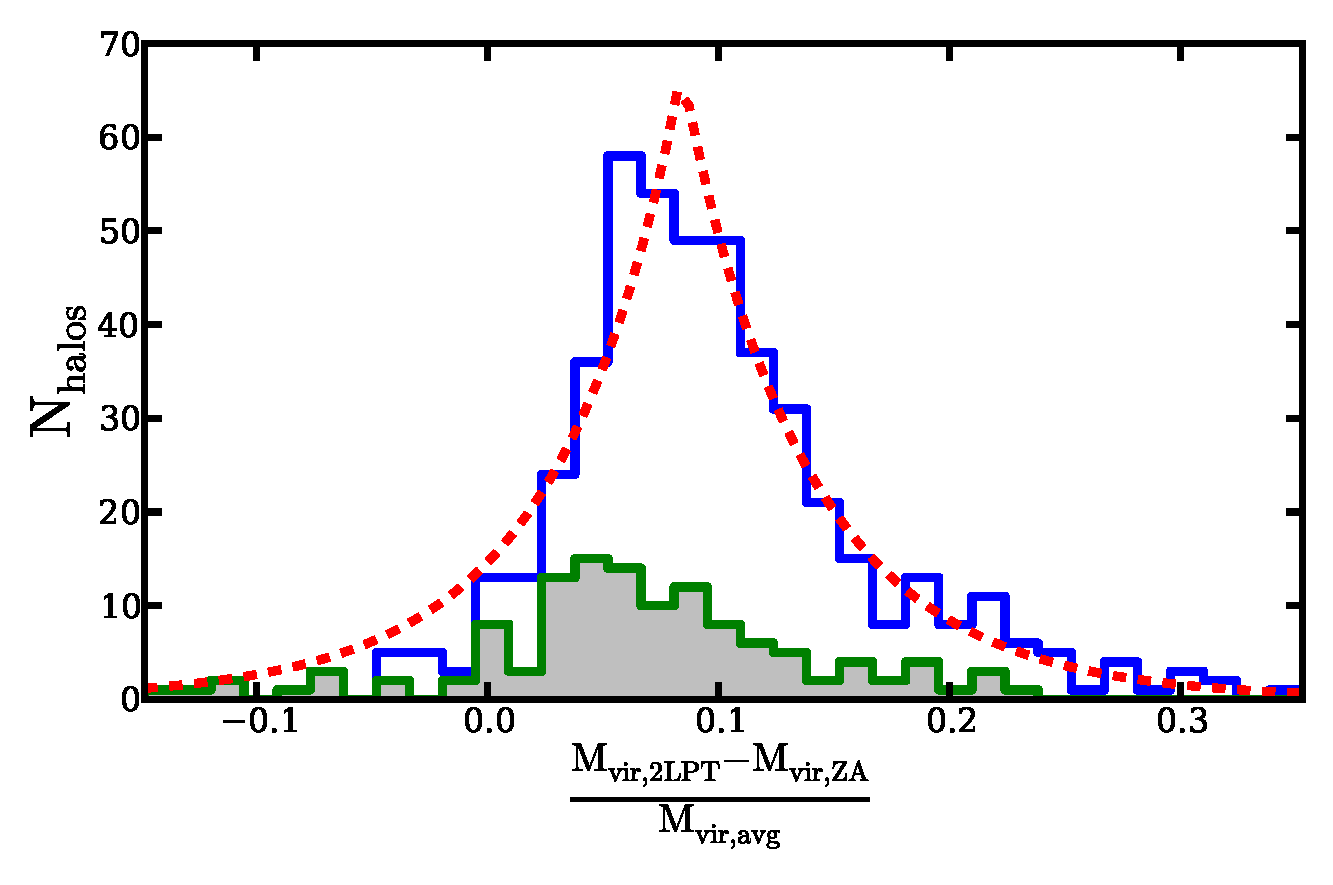
\includegraphics[width=0.48\linewidth]{analysis/diff-hist_Mvir_snap040_(0.0-1.0).eps}
	\end{subfigure}
	~
	\begin{subfigure}{}
		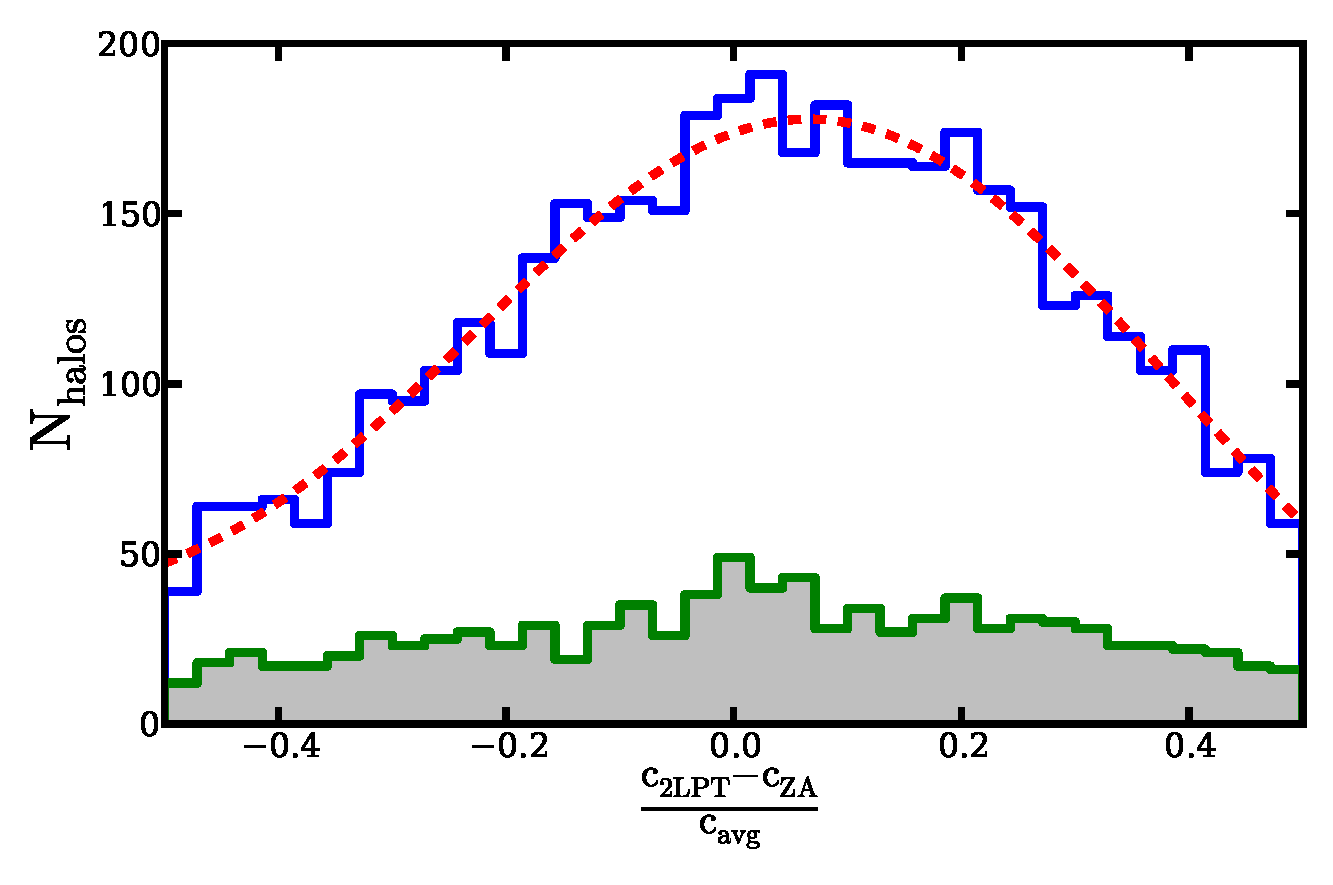
\includegraphics[width=0.48\linewidth]{analysis/diff-hist_c_snap040_(0.0-1.0).eps}
	\end{subfigure}
	\\
	\begin{subfigure}{}
		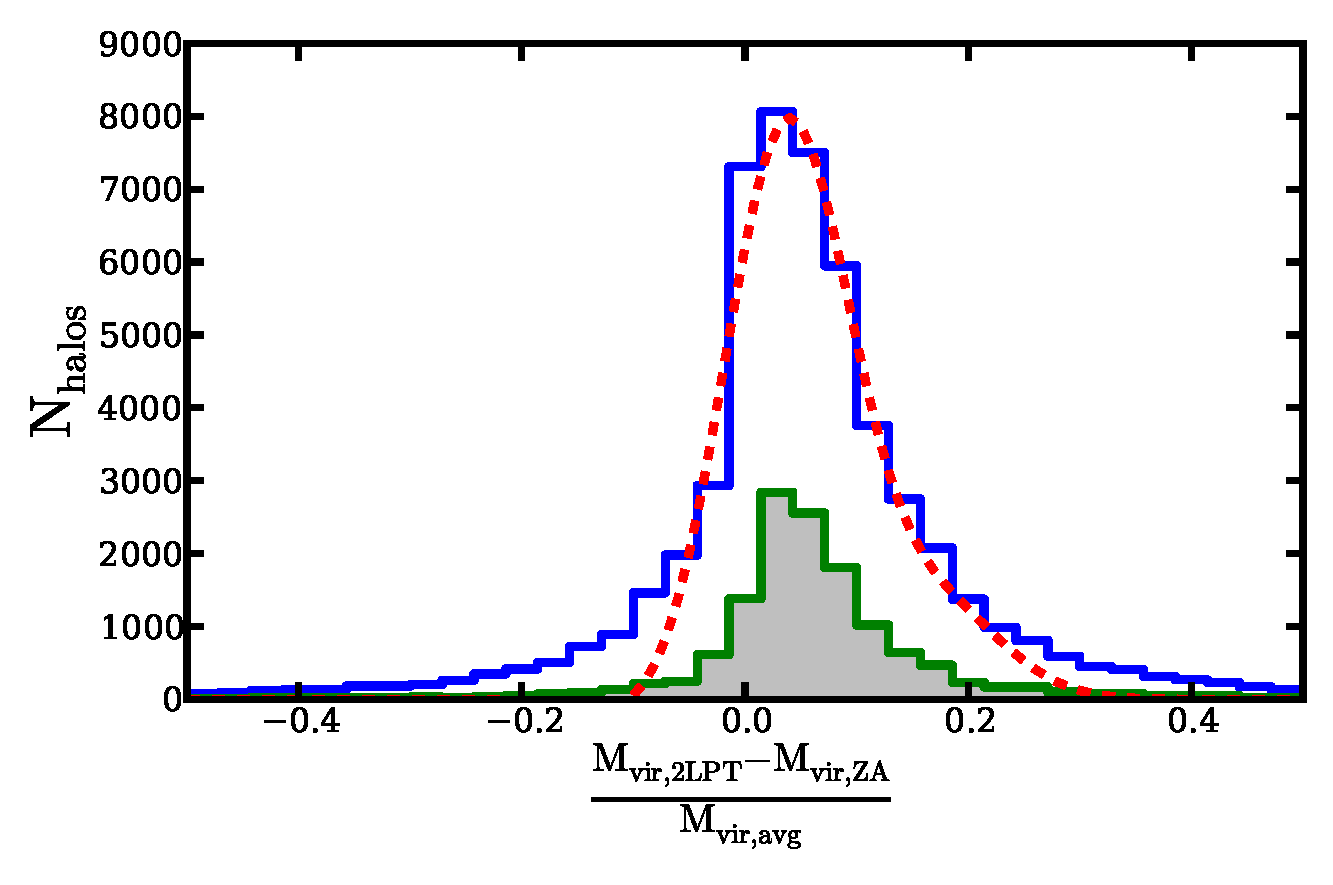
\includegraphics[width=0.48\linewidth]{analysis/diff-hist_Mvir_snap050_(0.0-1.0).eps}
	\end{subfigure}
	~
	\begin{subfigure}{}
		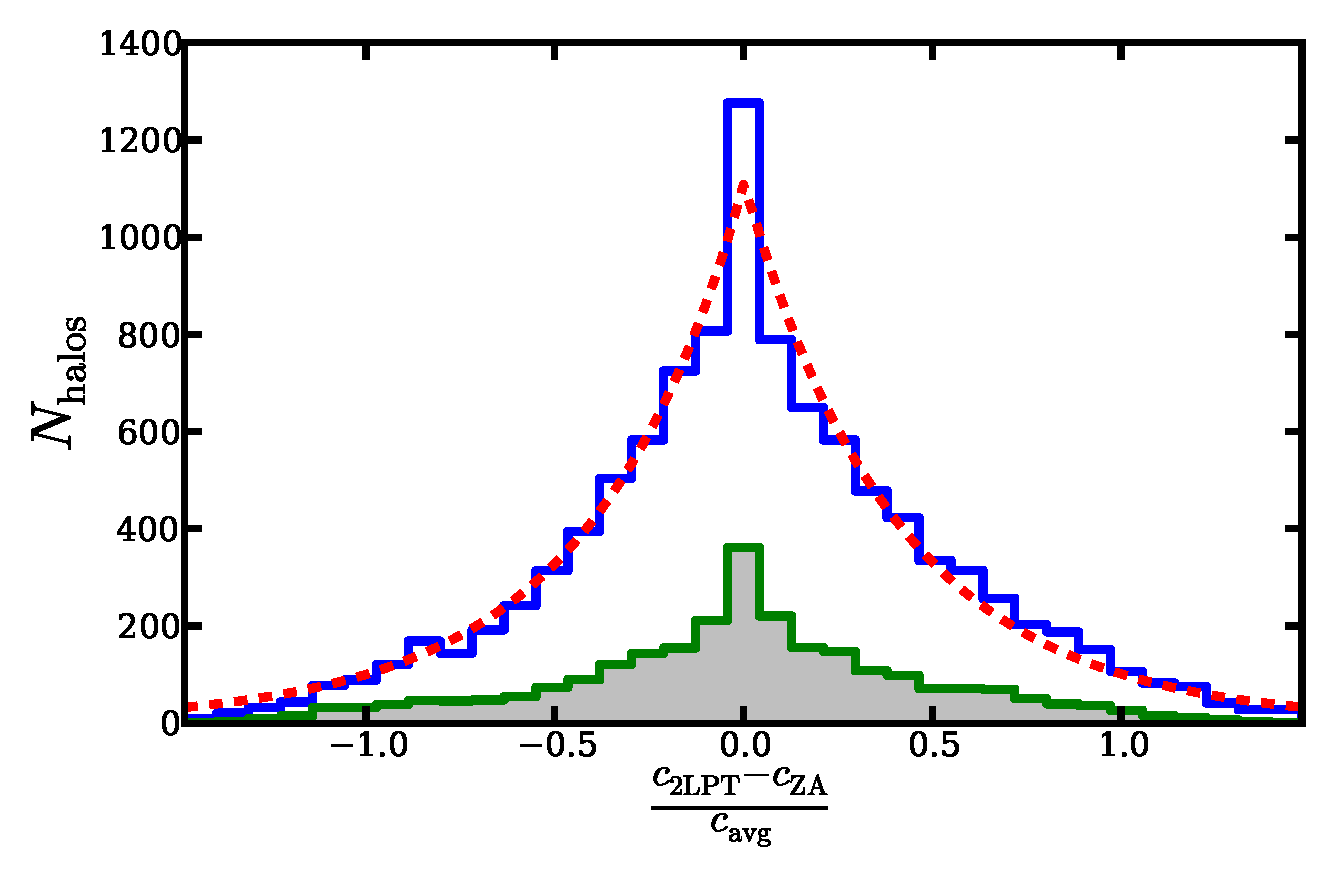
\includegraphics[width=0.48\linewidth]{analysis/diff-hist_c_snap050_(0.0-1.0).eps}
	\end{subfigure}
	\\
	\begin{subfigure}{}
		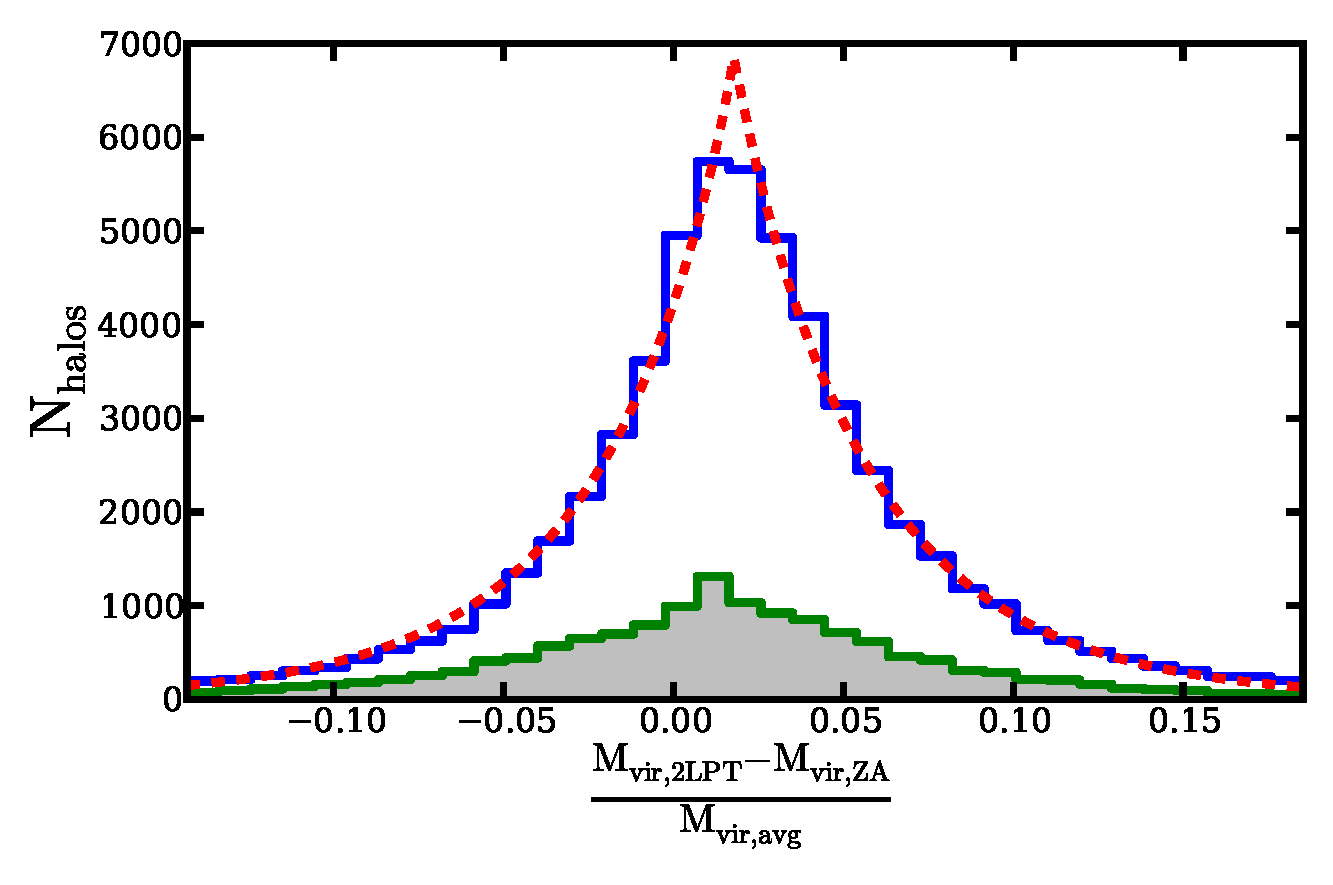
\includegraphics[width=0.48\linewidth]{analysis/diff-hist_Mvir_snap061_(0.0-1.0).eps}
	\end{subfigure}
	~
	\begin{subfigure}{}
		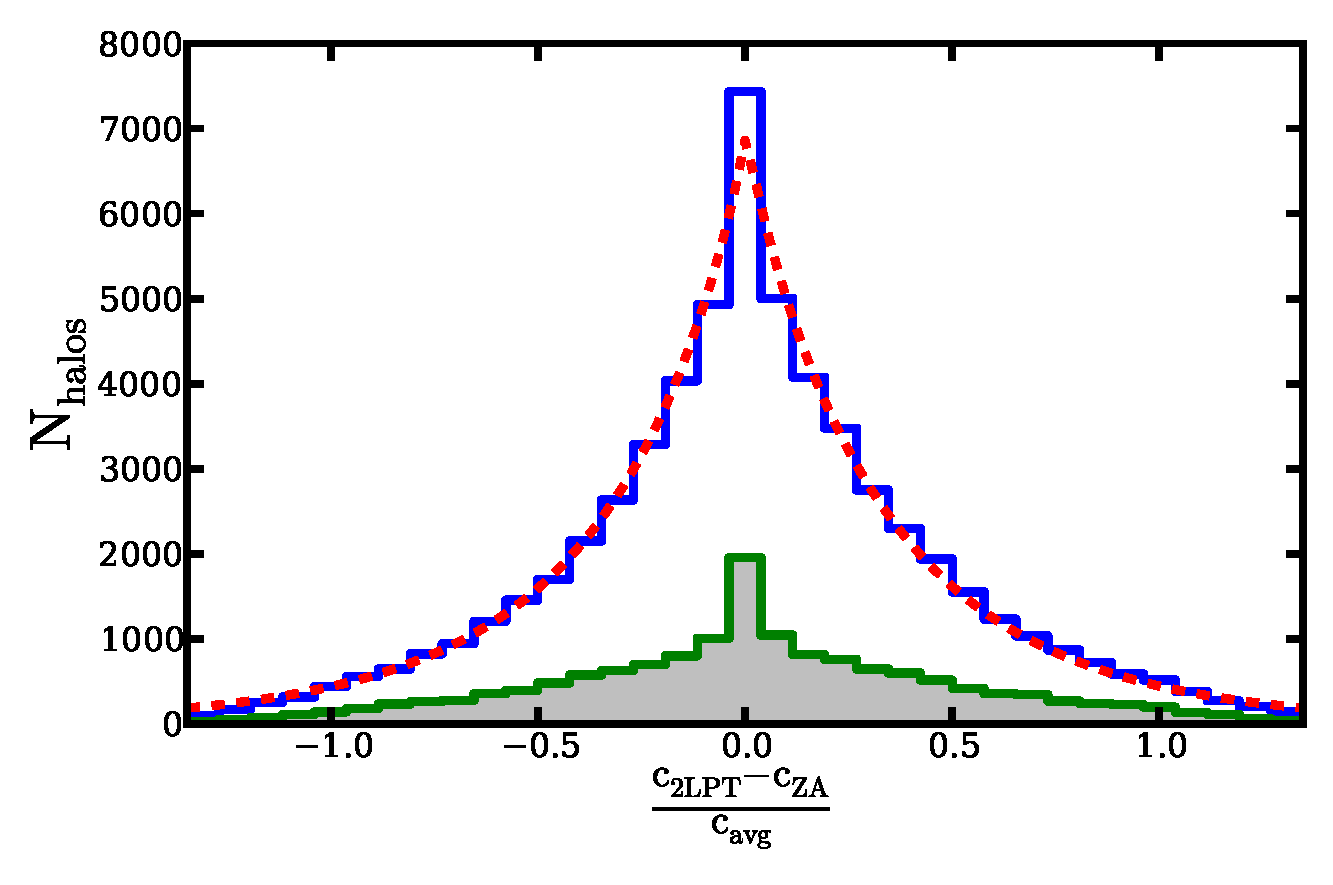
\includegraphics[width=0.48\linewidth]{analysis/diff-hist_c_snap061_(0.0-1.0).eps}
	\end{subfigure}
	\caption[Histograms of $\Delta M_{\mathrm{vir}}$ and $\Delta c$]{\footnotesize Histograms of $\Delta M_{\mathrm{vir}}$ (\textit{left column}) and $\Delta c$ (\textit{right column}) for snapshots at $z = 14.7$, $z = 10.3$, and $z = 6.0$ (\textit{top, middle, and bottom panels, respectively}).  The small gray-filled histograms count only the top 25\% most massive halos.  The main histograms are fit with a generalized normal distribution with parameters for mean, scale, and shape, overplotted as the red dashed line (see Equation~\ref{eq:analysis--methods--generalized_normal}).}
	\label{fig:methods--analysis--diff-hist}
\end{figure*}



%:::::::::::::::::::::::::::::::::::::::::::::::::::::::::::::::::::::::::::::::
\subsubsection{Mass Quartiles}
\label{subsubsec:analysis--difference_histograms--mass_quartiles}
%:::::::::::::::::::::::::::::::::::::::::::::::::::::::::::::::::::::::::::::::


Text goes here.




%~~~~~~~~~~~~~~~~~~~~~~~~~~~~~~~~~~~~~~~~~~~~~~~~~~~~~~~~~~~~~~~~~~~~~~~~~~~~~~~
\subsection{Redshift Trends}
\label{subsec:analysis--redshift_trends}
%~~~~~~~~~~~~~~~~~~~~~~~~~~~~~~~~~~~~~~~~~~~~~~~~~~~~~~~~~~~~~~~~~~~~~~~~~~~~~~~


Up to this point, we have only considered one snapshot at a time.  While we have observed variations with redshift, this has not been explicitly quantified.  In this section, we consider the statistical quantities derived from the generalized normal distribution fits from the previous section as functions of redshift.  The code used for this analysis is listed in Appendix~\ref{app:redshift_trends}.



%:::::::::::::::::::::::::::::::::::::::::::::::::::::::::::::::::::::::::::::::
\subsubsection{Mean and Standard Deviation}
\label{subsubsec:analysis--redshift_trends--mean_stdev}
%:::::::::::::::::::::::::::::::::::::::::::::::::::::::::::::::::::::::::::::::


Representing the mean and standard deviation of the distributions is relatively straightforward.  For the fit generalized normal distributions, we record values for the mean, uncertainty in the mean, standard deviation, and uncertainty in the standard deviation.  We also record the mean and standard deviation of the underlying distribution as directly measured from the data.

In Figure~\ref{fig:methods--analysis--fit_trends_mean_stdev}, we plot the mean and standard deviation of the distributions for mass and concentration, as well as the rms value derived from the data, all as functions of redshift.  The mean is plotted as blue points with error bars, the standard deviation is plotted as two black dashed lines that represent $\mu \pm \sigma$, and the rms is plotted as a dotted green line.

\begin{figure*}[t]
	\centering
	\begin{subfigure}{}
		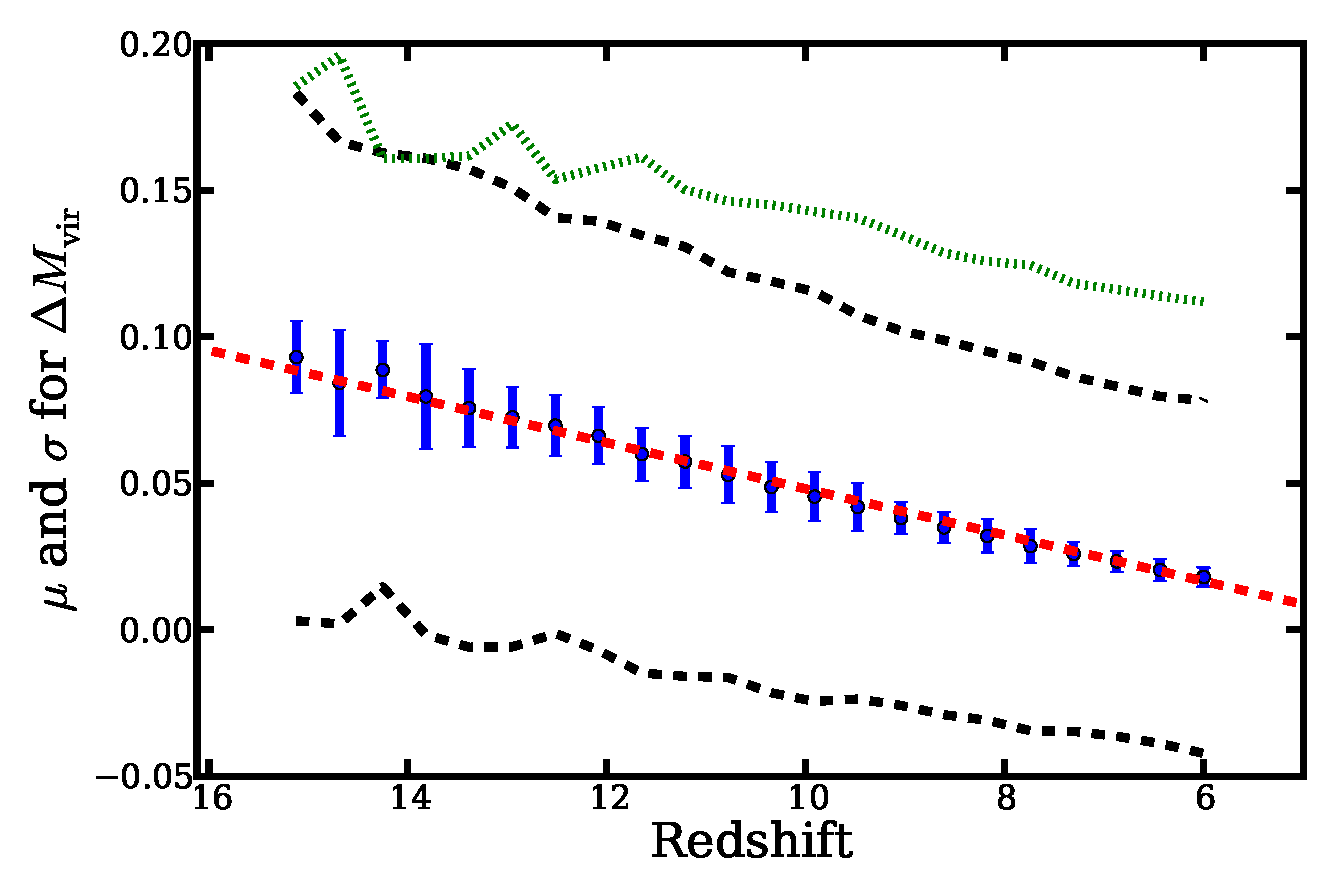
\includegraphics[width=0.75\linewidth]{analysis/mean_stdev_Mvir.eps}
	\end{subfigure}
	\\
	\begin{subfigure}{}
		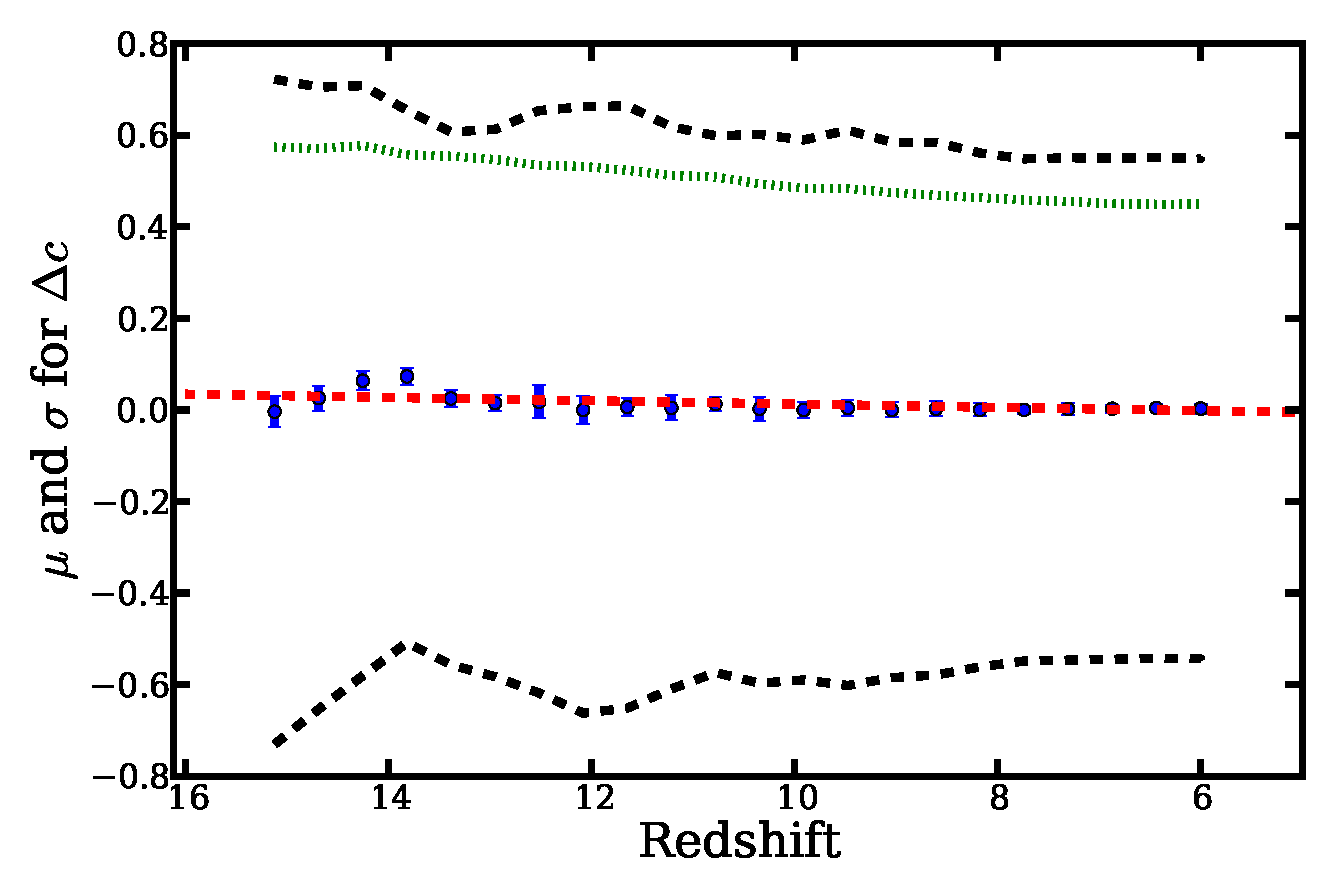
\includegraphics[width=0.75\linewidth]{analysis/mean_stdev_c_rockstar.eps}
	\end{subfigure}
	\caption[Mean, standard deviation, and rms as functions of redshift for generalized normal fits]{\footnotesize Mean, standard deviation, and rms as functions of redshift for $\Delta M_{\mathrm{vir}}$ (\textit{top}) and $\Delta c$ (\textit{bottom}).  The mean is plotted as blue points, $\mu \pm \sigma$ is plotted as the black dashed curves, and rms values are plotted as a green dotted curve.  The red dashed line is a linear fit to the mean.}
	\label{fig:methods--analysis--fit_trends_mean_stdev}
\end{figure*}

In this case, we wish to be conservative with the error bars on the mean.  Since we have a measurement for the mean both from the fitting distribution and the underlying data, we can incorporate both of these into our result.  The points plotted in Figure~\ref{fig:methods--analysis--fit_trends_mean_stdev} are the mean measured from the fit distribution, and the error bars are the uncertainty in the mean estimated from the least squares routine.  However, if the mean measured directly from the data falls outside the error bars, the error bars are expanded to encompass that measurement.  This is most often not a concern, as the means for most snapshots are very close together.  However, when there is a slight discrepancy between the fit and data values, the error bars will reflect this.



%:::::::::::::::::::::::::::::::::::::::::::::::::::::::::::::::::::::::::::::::
\subsubsection{Skew}
\label{subsubsec:analysis--redshift_trends--skew}
%:::::::::::::::::::::::::::::::::::::::::::::::::::::::::::::::::::::::::::::::


The generalized normal distributions we use to fit our $\Delta q$ histograms are symmetrical by definition and therefore have no inherent skew.  This was a simplifying assumption necessary to use a well-defined distribution as well as reduce the number of free parameters during fitting.  We do note, however, that the skew of our underlying data is often large enough to not be ignored.

Therefore, we need an alternate way to measure skew and its uncertainty.  We use the skew routine from the SciPy statistics library, which defines skew as
\begin{equation} \label{eq:skew_def}
	\gamma_{1} = \frac{ \mu_{3} }{ \mu_{2}^{3/2} },
\end{equation}
where $\mu_{m}$ are central moments given by
\begin{align} \label{eq:central_moments}
	\mu_{m} = E[(X - \mu)^{m}] &= \sum_{k} (x_{k} - \mu)^{m} p(x_{k}) \\
	                           &= \sum_{k=0}^{m} (-1)^{m - k} \binom{m}{k} \mu^{m - k} \mu_{k}',
\end{align}
with non-central moments $\mu_{m}'$ given by
\begin{equation} \label{eq:non-central_moments}
	\mu_{m}' = E[X^{m}] = \sum_{k} x_{k}^{m} p(x_{k}),
\end{equation}
where $p(x_{k})$ is the probability density function.  The skew is then measured from the entire halo sample for the three combined simulation boxes.  Uncertainty in skew is evaluated by taking the skew of the three boxes as independent measurements.  The results for skew as a function of redshift are plotted as blue curves for the $\Delta \Mvir$ and $\Delta c$ distributions in Figure~\ref{fig:methods--analysis--fit_trends_skew_kurtosis}.

\begin{figure*}[t]
	\centering
	\begin{subfigure}{}
		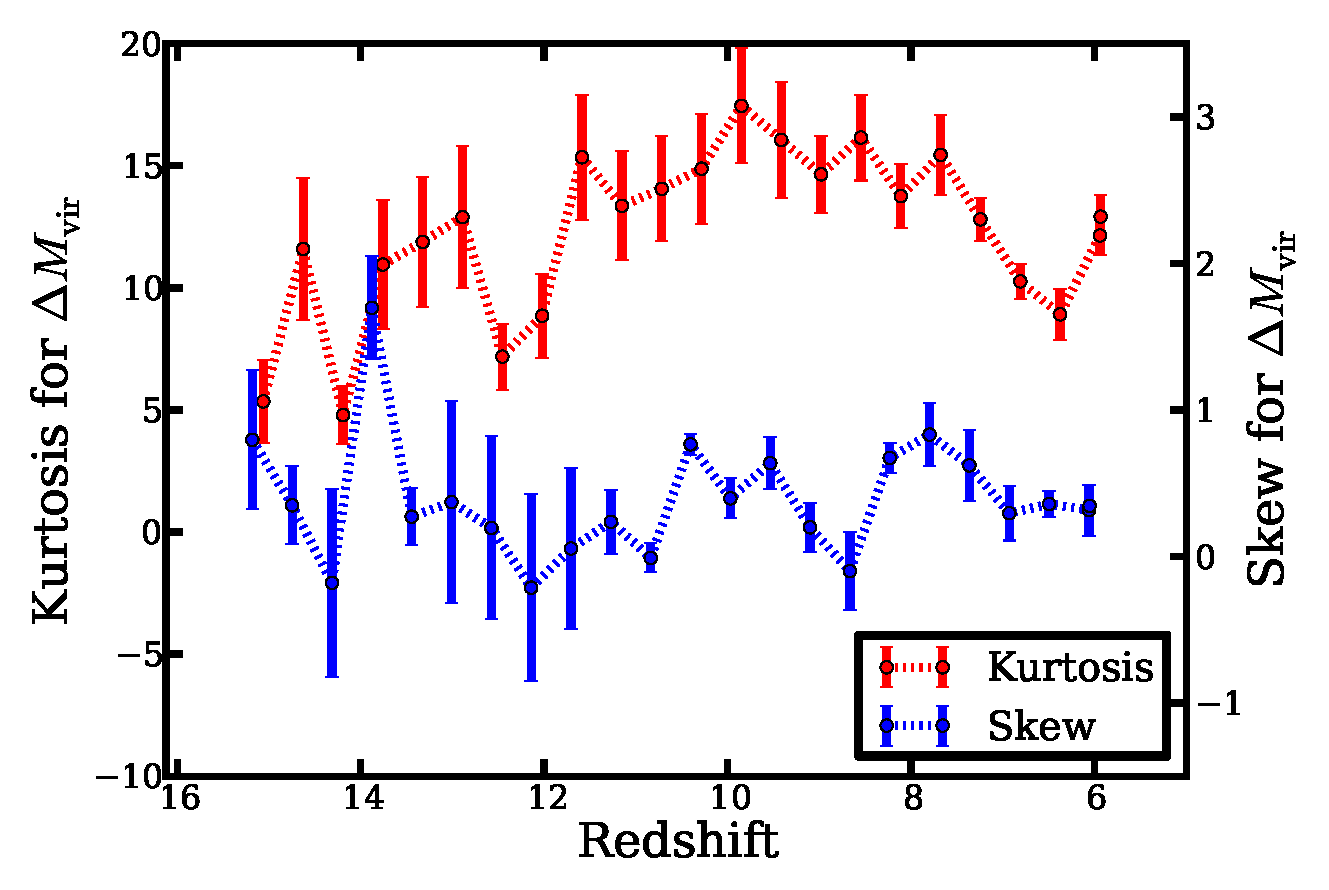
\includegraphics[width=0.75\linewidth]{analysis/skew_kurtosis_Mvir.eps}
	\end{subfigure}
	\\
	\begin{subfigure}{}
		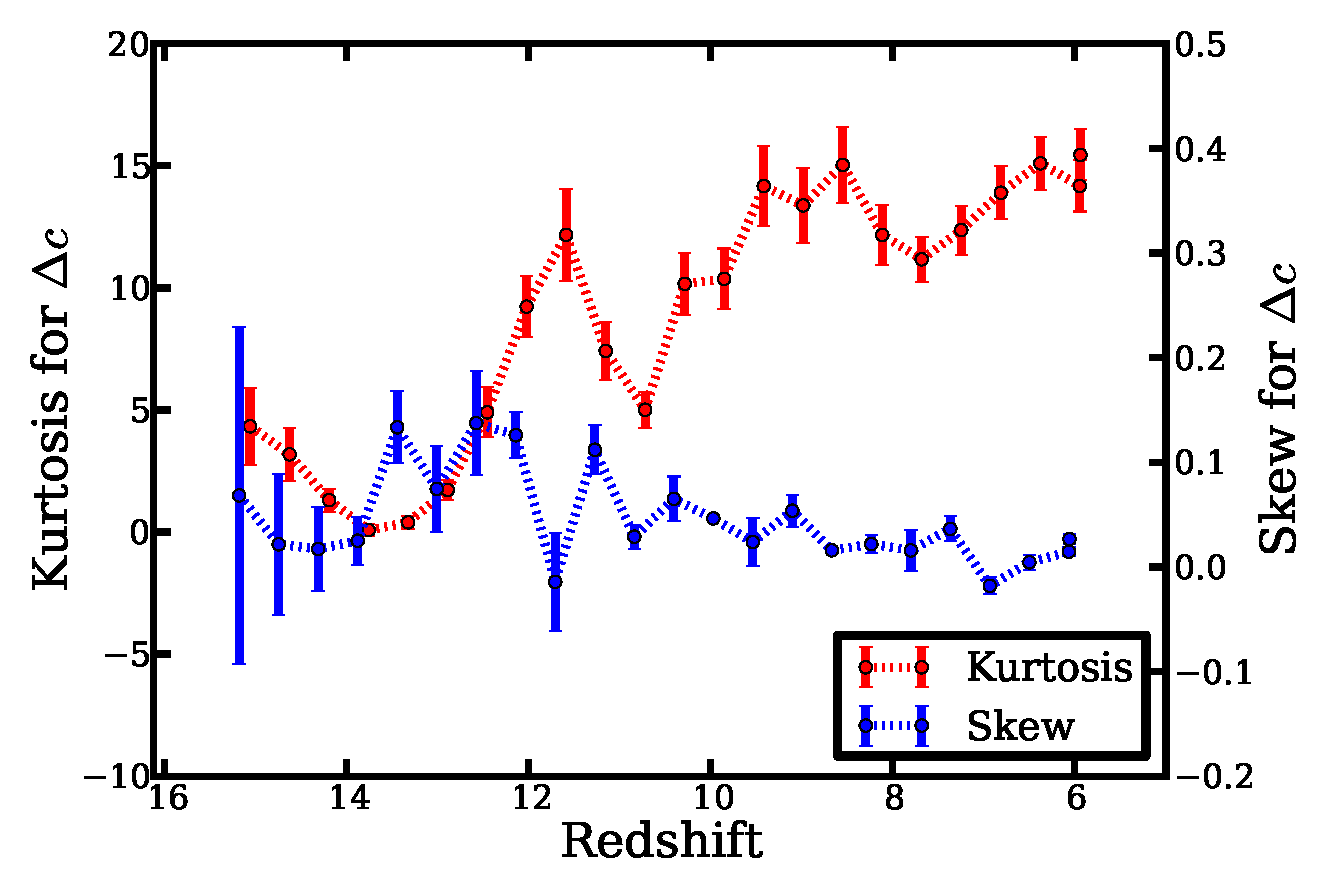
\includegraphics[width=0.75\linewidth]{analysis/skew_kurtosis_c_rockstar.eps}
	\end{subfigure}
	\caption[Skew and kurtosis as functions of redshift for generalized normal fits]{\footnotesize Skew (blue curve) and excess kurtosis (red curve) from generalized normal distribution fits as functions of redshift for $\Delta M_{\mathrm{vir}}$ (\textit{top}) and $\Delta c$ (\textit{bottom}).  For both plots, the left axis is the scale for kurtosis and the right axis is the scale for skew.}
	\label{fig:methods--analysis--fit_trends_skew_kurtosis}
\end{figure*}



%:::::::::::::::::::::::::::::::::::::::::::::::::::::::::::::::::::::::::::::::
\subsubsection{Kurtosis}
\label{subsubsec:analysis--redshift_trends--kurtosis}
%:::::::::::::::::::::::::::::::::::::::::::::::::::::::::::::::::::::::::::::::


Variable kurtosis is a fundamental part of the generalized normal distribution, so we may therefore derive the kurtosis directly from the fit distribution parameters.  The generalized normal distribution is defined in terms of a shape parameter $\beta$, which does introduce some complexity in the conversion to kurtosis.  The shape parameter is converted to excess kurtosis by way of Equation~\ref{eq:kurtosis}.  As this definition includes the Gamma function, a number of steps are required to convert the uncertainty in shape parameter to the uncertainty in kurtosis, which we outline below.

The standard deviation of a function $f(x_{1},x_{2},\dots,x_{n})$ is, in general, given by
\begin{equation} \label{eq:general_stdev}
	s_{f} = \sqrt{\sum_{x} \left( \frac{\partial f}{\partial x} \right)^{2} s_{x}^{2}}
\end{equation}
with summation over all independent variables $x$.  The generalized normal distribution
\begin{equation} \label{eq:generalized_normal}
	f(x) = \frac{\beta}{2 \alpha \Gamma(1/\beta)} e^{-(|x - \mu| / \alpha)^{\beta}}
\end{equation}
with mean $\mu$, scale parameter $\alpha$, and shape parameter $\beta$, has excess kurtosis
\begin{equation} \label{eq:kurtosis}
	\gamma_{2} = \frac{\Gamma(5/\beta) \Gamma(1/\beta)}{\Gamma(3/\beta)^{2}} - 3.
\end{equation}
The gamma function
\begin{equation} \label{eq:gamma_function}
	\Gamma(x) = \int_{0}^{\infty} t^{x-1} e^{-t} \dd t
\end{equation}
has the first derivative
\begin{equation} \label{eq:gamma_prime}
	\Gamma'(x) = \Gamma(x) \psi_{0}(x)
\end{equation}
where the digamma function $\digamma$ is the derivative of the logarithm of the gamma function and is given by
\begin{equation} \label{eq:digamma}
	\digamma(x) = \int_{0}^{\infty} \left( \frac{e^{-t}}{t} - \frac{e^{-xt}}{1 - e^{-t}} \right) \dd t
\end{equation}
if the real part of $x$ is positive.

We now apply \eqref{eq:general_stdev} to \eqref{eq:kurtosis} to find the standard deviation of the excess kurtosis:
\begin{align} \label{eq:kurt_err_partial1}
	s_{\gamma_{2}} &= \sqrt{ \left( \frac{\diff \gamma_{2}}{\diff \beta} \right)^{2} s_{\beta}^{2} } \\
		&= s_{\beta} \frac{\diff \gamma_{2}}{\diff \beta} \\
		&= s_{\beta} \frac{\diff}{\diff \beta} \left[ \frac{\Gamma(5/\beta) \Gamma(1/\beta)}{\Gamma(3/\beta)^{2}} - 3 \right].
\end{align}
Making the substitution $x = 1 / \beta$ and $\diff x = - 1 / \beta^{2} \dd \beta$, taking the derivative, and doing a bit of algebra, we have:
\begin{align} \label{eq:kurt_err_partial2}
	s_{\gamma_{2}} &= s_{\beta} \frac{\diff \gamma_{2}}{\diff x} \frac{\diff x}{\diff \beta} \\
		&= s_{\beta} \left( -\frac{1}{\beta^{2}} \right) \frac{\diff}{\diff x} \left[ \frac{\Gamma(5x) \Gamma(x)}{\Gamma(3x)} - 3 \right] \\
		&= -s_{\beta} x^{2} \left\{ \frac{\Gamma(3x)^{2} \frac{\diff}{\diff x} [\Gamma(5x) \Gamma(x)] - \Gamma(5x) \Gamma(x) \frac{\diff}{\diff x} [\Gamma(3x)^{2}]}{\Gamma(3x)^{4}} \right\} \\
		&= -s_{\beta} \frac{x^{2}}{\Gamma(3x)^{4}} \left\{ \Gamma(3x)^{2} [5\Gamma(5x) \digamma(5x) \Gamma(x) + \Gamma(5x) \Gamma(x) \digamma(x)] - \Gamma(5x) \Gamma(x) [6\Gamma(3x)^{2} \digamma(3x)] \right\} \\
		&= s_{\beta} \frac{x^{2}}{\Gamma(3x)^{4}} \left\{ 6\Gamma(5x) \Gamma(3x)^{2} \Gamma(x) \digamma(3x) - \Gamma(5x) \Gamma(3x)^{2} \Gamma(x) [5\digamma(5x) + \digamma(x)] \right\} \\
		&= s_{\beta} \frac{x^{2}}{\Gamma(3x)^{4}} \left\{ \Gamma(5x) \Gamma(3x)^{2} \Gamma(x) [6\digamma(3x) - 5\digamma(5x) - \digamma(x)] \right\} \\
		&= s_{\beta} x^{2} \frac{\Gamma(5x) \Gamma(x)}{\Gamma(3x)^{2}} [6\digamma(3x) - 5\digamma(5x) - \digamma(x)].
\end{align}
Substituting back in for $x$ and recognizing an occurance of $\gamma_{2}$, we have the result
\begin{equation} \label{eq:kurt_err}
	s_{\gamma_{2}} = s_{\beta} \frac{1}{\beta^{2}} \left( \gamma_{2} + 3 \right) \left[ 6 \digamma(3/\beta) - 5 \digamma(5/\beta) - \digamma(1/\beta) \right]
\end{equation}
with which we can find the uncertainty in the kurtosis given the value and uncertainty of the shape parameter $\beta$.

With a method of determining the uncertainty in kurtosis established, we may now examine the results.  In Figure~\ref{fig:methods--analysis--fit_trends_skew_kurtosis}, we plot the kurtosis and associated uncertainties as a function of redshift as red curves for distributions of $\Delta \Mvir$ and $\Delta c$.




%~~~~~~~~~~~~~~~~~~~~~~~~~~~~~~~~~~~~~~~~~~~~~~~~~~~~~~~~~~~~~~~~~~~~~~~~~~~~~~~
\subsection{Mass Trends}
\label{subsec:analysis--mass_trends}
%~~~~~~~~~~~~~~~~~~~~~~~~~~~~~~~~~~~~~~~~~~~~~~~~~~~~~~~~~~~~~~~~~~~~~~~~~~~~~~~


Text goes here.



%:::::::::::::::::::::::::::::::::::::::::::::::::::::::::::::::::::::::::::::::
\subsubsection{Binning and Plotting}
\label{subsubsec:analysis--mass_trends--binning_plotting}
%:::::::::::::::::::::::::::::::::::::::::::::::::::::::::::::::::::::::::::::::


Text goes here.



%:::::::::::::::::::::::::::::::::::::::::::::::::::::::::::::::::::::::::::::::
\subsubsection{Fitting}
\label{subsubsec:analysis--mass_trends--fitting}
%:::::::::::::::::::::::::::::::::::::::::::::::::::::::::::::::::::::::::::::::


Text goes here.




%~~~~~~~~~~~~~~~~~~~~~~~~~~~~~~~~~~~~~~~~~~~~~~~~~~~~~~~~~~~~~~~~~~~~~~~~~~~~~~~
\subsection{Alternate Difference Distributions}
\label{subsec:analysis--alt_diff_dist}
%~~~~~~~~~~~~~~~~~~~~~~~~~~~~~~~~~~~~~~~~~~~~~~~~~~~~~~~~~~~~~~~~~~~~~~~~~~~~~~~


Text goes here.



%:::::::::::::::::::::::::::::::::::::::::::::::::::::::::::::::::::::::::::::::
\subsubsection{Equivalent Displacement}
\label{subsubsec:analysis--alt_diff_dist--equiv_displacment}
%:::::::::::::::::::::::::::::::::::::::::::::::::::::::::::::::::::::::::::::::


Text goes here.



%:::::::::::::::::::::::::::::::::::::::::::::::::::::::::::::::::::::::::::::::
\subsubsection{Redshift Trends}
\label{subsubsec:analysis--alt_diff_dist--trends}
%:::::::::::::::::::::::::::::::::::::::::::::::::::::::::::::::::::::::::::::::


Text goes here.




